\documentclass[12pt]{article}

\usepackage{booktabs}% http://ctan.org/pkg/booktabs
\usepackage[utf8]{inputenc}
\usepackage{changepage}
\usepackage{pgfplots}
\usepackage{amssymb}
\usepackage{xcolor}
\usepackage{hyperref}
\usepackage{listings}
\usepackage[T1]{fontenc}
\usepackage[utf8]{inputenc}
\usepackage{adjustbox}
\usepackage{biblatex}
\lstset{
  language=Python,
  numbers=left,
  numberstyle=\tiny,
  stepnumber=1,
  numbersep=5pt,
  tabsize=4,
  basicstyle=\ttfamily,
  columns=fullflexible,
  keepspaces,
}
\hypersetup{
    colorlinks,
    citecolor=black,
    filecolor=black,
    linkcolor=black,
    urlcolor=black
}

% Set page size and margins
% Replace `letterpaper' with `a4paper' for UK/EU standard size
\usepackage[letterpaper,top=2cm,bottom=2cm,left=3cm,right=3cm,marginparwidth=1.75cm]{geometry}

% Useful packages
\usepackage{amsmath}
\usepackage{mathtools}
\usepackage{graphicx}

\title{Appunti di Algebra lineare e Geometria}
\date{A.A 2022-20}

\newenvironment{para}{\begin{adjustwidth}{13mm}{}}{\end{adjustwidth}}

\newcommand\tab[1][1cm]{\hspace*{#1}}

\newcommand{\tabitem}{\llap{\textbullet}}
\newcommand{\Hsquare}{%
\text{\fboxsep=-.2pt\fbox{\rule{0pt}{1ex}\rule{1ex}{0pt}}}%
}

\newtheorem{Definizione}{Definizione}[subsection]
\newtheorem{Lemma}{Lemma}[subsection]
\newtheorem{Teorema/Definizione}{Teorema/Definizione}[subsection]
\newtheorem{Corollario}{Corollario}[subsection]
\newtheorem{Teorema}{Teorema}[subsection]
\newtheorem{Proposizione}{Proposizione}[subsection]
\newtheorem{Notazione}{Notazione}[subsection]
\newtheorem{Commento}{Commento}[subsection]
\newtheorem{Dimostrazione}{Dimostrazione}[subsection]
\newtheorem{Osservazione}{Osservazione}[subsection]


\begin{document}

\begin{figure}
\centering

\includegraphics[width=0.35\textwidth]{Immagini/Logo scienze bicocca.png}
\end{figure}

\vspace{10cm}
\date{A.A. 2022-2023}
\maketitle

\newpage

\tableofcontents
\newpage

\section{Spazi vettoriali}
\begin{para}
\begin{Definizione}[Campo]
Un campo $\mathbb{K}$ è un insieme dotato di due operazioni, individuate con $+ \; e \; \cdot$, che soddisfano le seguenti proprietà:\newline
$1)$ $(\mathbb{K}, +)$ è un gruppo abeliano:
\begin{itemize}
    \item $a+(b+c) = (a+b)+c \; \forall a,b,c \in \mathbb{K}$ (proprietà associativa della somma)
    \item $a+0 = 0+a = a \; \forall a \in \mathbb{K}$ (esistenza dell'elemento neutro)
    \item $\forall a \in \mathbb{K} \; \exists -a \in \mathbb{K} | -a+a = a+(-a) = 0$ (esistenza dell'opposto)
    \item $a+b = b+a \; \forall a,b \in \mathbb{K}$ (proprietà commutativa)
\end{itemize}
$2)$ $(\mathbb{K} \textbackslash \{0\}, \cdot)$ è un gruppo abeliano:
\begin{itemize}
    \item $a\cdot(b\cdot c) = (a\cdot b)\cdot c \; \forall a,b,c \in \mathbb{K}$ (associatività)
    \item $a \cdot 1 = 1 \cdot a = a$ (Elemento neutro)
    \item $\forall a \in \mathbb{K} \textbackslash \{0\} \; \exists a^{-1} = 1/a \in \mathbb{K} \textbackslash \{0\} | a \cdot a^{-1} = a^{-1} \cdot a = 1$ (esistenza dell'opposto)
    \item $a \cdot b = b \cdot a \; \forall a,b \in \mathbb{K}$ (commutatività)
\end{itemize}
$3)$ Il prodotto gode della proprietà distributiva rispetto alla somma: $$a \cdot (b+c) = (a\cdot b) + (a \cdot c) \; \forall a,b,c \in \mathbb{K}$$
\end{Definizione}
\begin{Definizione}[Spazio vettoriale]
Diremo che V è uno spazio vettoriale su campo $\mathbb{K}$ se esistono 2 operazioni su V che godono delle seguenti proprietà:
\end{Definizione}
Operazione 1) (Operazione interna): $+ : V\times V \rightarrow V$
\begin{itemize}
  \item $\exists0_v\in V | 0_v + \underline{v} = \underline{v} \forall v \in V$ (Elemento neutro)
  \item $\forall \underline{v} \in V, \exists -\underline{v} \in V | \underline{v} + (-\underline{v}) = \underline{0}$ (opposto di \underline{v})
  \item $(\underline{v_1} + \underline{v_2})+\underline{v_3} = \underline{v_1}+(\underline{v_2}+\underline{v_3}) \forall \underline{v_1}, \underline{v_2 },\underline{v_3} \in V$ (Associatività)
  \item $\underline{v_1} + \underline{v_2} = \underline{v_2} + \underline{v_1} \forall \underline{v_1}, \underline{v_2} \in V$ (commutatività)
\end{itemize}
Operazione 2) (Operazione esterna): $\cdot : \mathbb{K}\times V \rightarrow V$
\begin{itemize}
  \item $(\lambda_1 +_\mathbb{K} \lambda_2) \cdot \underline{v} = \lambda_1 \underline{v} + \lambda_2 \underline{v} $ (distributività per uno scalare)
  \item $(\underline{v_1} +_V \underline{v_2})\cdot \lambda = \lambda \underline{v_1} + \lambda \underline{v_2}$ (distributività per uno scalare della somma di vettori)
  \item $(\lambda_1 \cdot_\mathbb{K} \lambda_2)\underline{v} = \lambda_1(\lambda_2\underline{v})$ (omogeneità)
  \item $1 \cdot \underline{v} = \underline{v}$ (elemento neutro del prodotto)
\end{itemize}

\begin{Teorema}[Legge di cancellazione della somma]
Dall'uguaglianza \newline $\underline{v}+\underline{w_1} = \underline{v}+\underline{w_2}$ segue che $\underline{w_1} = \underline{w_2}$
\end{Teorema}

\begin{Dimostrazione}
Per dimostrare la legge di cancellazione, sommiamo -$\underline{v}$ a entrambi i membri di $\underline{v}+\underline{w_1} = \underline{v}+\underline{w_2}$, ottenendo: \newline
$$-\underline{v} + (\underline{v}+\underline{w_1}) = -\underline{v} + (\underline{v}+\underline{w_2})$$
Per la proprietà associativa, il primo membro è uguale a:
$$(-\underline{v}+\underline{v})+\underline{w_1} = \underline{0}+\underline{w_1}=\underline{w_1}$$
Per lo stesso motivo, il membro di destra è uguale al $\underline{w_2}$, quindi si ha che $\underline{w_1} = \underline{w_2}$
\end{Dimostrazione}

\begin{Corollario}
Come conseguenza logica della dimostrazione, si ha che il vettore opposto di $\underline{v}$ è univocamente determinato da $\underline{v}$. Infatti, se $\underline{w_1}$ e $\underline{w_2}$ sono due vettori opposti di $\underline{v}$, allora: $$\underline{v}+\underline{w_1} = \underline{0} = \underline{w_2} + \underline{v}$$ e dalla legge di cancellazione, segue che $\underline{w_1} = \underline{w_2}$
\end{Corollario}

\begin{Proposizione}
La differenza $\underline{v}-\underline{w}$ di due vettori si definisce ponendo $$\underline{v}-\underline{w} = \underline{v} + (-\underline{w})$$
Naturalmente, $\underline{w} + (\underline{v}-\underline{w}) = v$: analogamente al caso dell'aritmeitca, la differenza tra $\underline{v}$ e $\underline{w}$ è quel vettore che sommato a $\underline{w}$ da come risultato $\underline{v}$.
\end{Proposizione}

\begin{Teorema} [Legge di annullamento del prodotto per uno scalare]
Il vettore $t\underline{v}$ è nullo $\Leftrightarrow$ $t = 0$ oppure $\underline{v} = \underline{0}$
\end{Teorema}
\begin{Dimostrazione}
Mostriamo che $0\underline{v} = \underline{0}$ per ogni vettore $\underline{v}$: infatti $$\underline{v} + 0\underline{v}=1\underline{v}+0\underline{v}=(1+0)\underline{v}=1\underline{v}=\underline{v}=\underline{v}+0$$
e quindi $0\underline{v}=\underline{0}$ per la legge di cancellazione della somma. \newline
Mostriamo che $t\underline{0} = \underline{0}$ per ogni scalare t: infatti per ogni vettore $\underline{v}$: $$t\underline{0}=t(\underline{0}+\underline{0}) = t\underline{0}+t\underline{0}$$ e sommando $-t\underline{0}$ otteniamo $\underline{0} = t\underline{0}$.
\newline Mostriamo, viceversa, che, da $t\underline{v} =  \underline{0}$ segue $t = 0$ oppure $\underline{v} = \underline{0}$. Infatti, se $t\underline{v}=\underline{0}$ ma $t \neq 0$ si ha che: $$\underline{0} = t^{-1}\underline{0} = t^{-1}(t\underline{v})=(t \cdot t^{-1})\underline{v} = 1\underline{v} = \underline{v}$$ Infine osserviamo come il vettore opposto $-\underline{v}$ coincide con il prodotto $(-1)\underline{v}$ del vettore $\underline{v}$ con lo scalare -1. Infatti:
$$\underline{v} + (-1)\underline{v} = 1\underline{v} + (-1)\underline{v} = (1 + (-1))\underline{v} = 0\underline{v} = \underline{0}$$
\end{Dimostrazione}
Riassumendo, in uno spazio vettoriale è definita un'operazione di somma che gode delle stesse proprietà dell'usuale somma di numeri: rispetto alla somma, le regole per il calcolo per i vettori sono le stesse che valgono per i numeri. Anche se non è definito il prodotto di due vettori, un vettore può essere moltiplicato per uno scalare t; se t non è nullo, si può dividere un vettore per t (moltiplicandolo per $t^{-1}$)
\newpage
\subsection{Sottospazi vettoriali}
\begin{Definizione}[Sottospazio vettoriale]
Sia V uno spazio vettoriale su campo $\mathbb{K}$ e $W \subset V$. Diremo che W è un sottopsazio vettoriale di V se W è uno spazio vettoriale rispetto alle operazioni di somma e prodotto per uno scalare di V. Questo è il caso se e solo se W soddisfa le seguenti proprietà:
\begin{itemize}
    \item  Il vettore nullo $\underline{0_V}$ appartiene a W
    \item W è chisuo rispetto alla somma, cioè se $\underline{w_1}+\underline{w_2}\in W \; \forall\underline{w_1},\underline{w_2}\in W$
    \item W è chiuso rispetto al prodotto per uno scalare, cioè se $\lambda \underline{w}\in W \; \forall\underline{w}\in W$ e $\forall \lambda \in \mathbb{K}$
\end{itemize}
\end{Definizione}

\begin{Osservazione}
Se un sottoinsieme W di V è chiuso rispetto al prodotto scalare e contiene un vettore $\underline{v}$, allora contiene anche il vettore nullo perché $0\underline{v}=\underline{0}$. Nelle proprietà che caratterizzano un sottospazio si può quindi sostituire la 1° con la richiesta che W non sia vuoto.
\end{Osservazione}

\begin{Proposizione}
I sottospazi vettoriali di un insieme V si indicano con "<"
\end{Proposizione}
\begin{Proposizione}
    Sia $V < \mathbb{R}^n$ e sia $dim(V) = k$. Il più piccolo sottospazio vettoriale contenente $\mathbb{R}^n/V$ ha dimensione $n-k$
\end{Proposizione}
\subsubsection{Sottospazi vettoriali di $\mathbb{R}^2$}
In $\mathbb{R}^2$ abbiamo i seguenti spazi vettoriali:
\begin{itemize}
    \item \{$\underline{0_v}$\}
    \item Retta per l'origine
    \item $\mathbb{R}^2$ è sottospazio vettoriale di se stesso
\end{itemize}

\subsubsection{Span e generazione di spazi vettoriali}
Dato $S \subset V$ spazio vettoriale, si indica con $<S> \; < V$ il più piccolo sottospazio vettoriale di V che contiene S (Si dice anche "il più piccolo spazio vettoriale generato da S"). Si dimostra che:  

$$<S> = \{\sum_{i = 1}^{n} \lambda_i \cdot \underline{z_i} | \lambda_i \in \mathbb{R}, \underline{z_i} \in S, n\in \mathbb{N}\} $$


\section{Dipendenza e indipendenza lineare}
\begin{Definizione}[Combinazione lineare]
$\sum_{i = 1}^{n} \lambda_i \cdot \underline{z_i}$ si chiama "combinazione lineare dei vettori $\{\underline{z_i}\}_{i=1,...,n}$
\end{Definizione}
\begin{Definizione} [Dipendenza e indipendenza lineare]
Sia $S \subset V$ spazio vettoriale. I vettori di S si dicono "linearmente dipendenti" $\Leftrightarrow \exists \underline{w} \in S, S_w = \{\underline{z_1}, ... \underline{z_h}\} \subset S | w = \sum_{i = 1}^{n} \lambda_i \cdot \underline{z_i}, \lambda_i \in \mathbb{K}$. In caso contrario, i vettori si dicono "linearmente indipendenti".
\end{Definizione}
\begin{Lemma}
$S \subset V$ è un insieme di vettori "linearmente indipendenti" $\Leftrightarrow \sum_{i = 1}^{n} \lambda_i \cdot \underline{z_i} = \underline{0_v} \Rightarrow \lambda_i = 0 \; \forall i$ Ciò deve valere $\forall n \in \mathbb{N} \; e \; \{\underline{z_i}\} \subset S$
\end{Lemma}

\begin{Dimostrazione}[Lemma 2.1]\; \newline
$\Rightarrow$: $S \subset V$ è un insieme di vettori linearmente indipendenti. Vogliamo dimostrare che, se $\{z_i\}\subset S$ e $\sum_{i=1}^n{\lambda_i \cdot \underline{z_i}}=\underline{0_V}$ allora $\lambda_i = 0 \; \forall i$. Per assurdo, supponiamo che $\sum_{i=1}^n{\lambda_i \cdot \underline{z_i}}=\underline{0_V}$ ma $\exists h| \lambda_h \neq 0$. Allora:
$$\lambda_h \underline{z_h} = -\sum_{j\neq h} {\lambda_j \underline{z_j}} \Rightarrow \newline
(\lambda_h ^-1 \cdot \lambda_h)\underline{z_h} = -\lambda_h^-1 \cdot \sum_{j\neq h} {\lambda_j \underline{z_j}} \Rightarrow$$
$$\underline{z_h} = -\lambda_h^-1 \cdot \sum_{j\neq h} {\lambda_j \underline{z_j}} = \sum_{j\neq h} {\lambda_h^-1\lambda_j \underline{z_j}}$$
L'ultimo risultato enuncia che il vettore è il risultato di una combinazione lineare dei vettori di S diversi da $\underline{z_h}$, il che è la definizione di dipendenza lineare. Quindi i vettori di $\{z_i\}_{i = 1,...,n}$ sono vettori linearmente dipendenti. \newline
$\Leftarrow$: Supponiamo che $\sum_{i=1}^n{\lambda_i \cdot \underline{z_i}}=\underline{0_V} \Rightarrow \lambda_i = 0 \; \forall i$. Dimostriamo che S è un insieme di vettori linearmente indipendenti. Supponiamo quindi che S siano vettori linearmente dipendenti; dimostriamo che:
$\exists \sum_{i=1}^n{\lambda_i \cdot \underline{z_i}}=\underline{0_V}$ con almeno un $\lambda_i \neq 0$. Per ipotesi, $\exists \underline{z_c} \in S | \underline{z_c} = \sum_{j=1}^m{\lambda_j \cdot \underline{z_j}}$ con $\underline{z_j} \neq \underline{z_c} \; \forall j$.
$$\underline{z_c} = \sum_{j=1}^n{\lambda_j \cdot \underline{z_j}}$$
$$\underline{0_V} = - \underline{z_c} + \sum_{j=1}^n{\lambda_j \cdot \underline{z_j}}$$
Il risultato esprime una combinazione lineare di vettori di S con almeno un $\lambda _i$ ($\lambda_c = -1)$
non nullo.
\end{Dimostrazione}
\begin{Osservazione}
Per abuso di linguaggio, si dice spesso che i vettori $\underline{v_1},...,\underline{v_d}$ sono linearmente (in)dipendenti se l'insieme $\{\underline{v_1},...,\underline{v_d}\}$ è linearmente (in)dipendente. Si tratta di un abuso di linguaggio perché la dipendenza lineare non è una proprietà die singoli vettori ma dell'insieme da essi formato. Dire che i vettori $\underline{v_1},...,\underline{v_d}$ sono linearmente indipendenti non significa che ognungo di essi ha la capacità di essere linearmente indipendente ma che tra i vettori non sussistono relazioni di dipendenza lineare.
\end{Osservazione}

\section{Basi}
\begin{Definizione}
Sia $W < V$. Ci sono 2 modi per "comunicare un sottospazio vettoriale":
\begin{itemize}
    \item Siccome $W \subset V, W = \{...\}$
    \item Sfruttiamo il fatto che W è un "sottospazio vettoriale" di V e quindi: \newline $<S> = W$ per qualche insieme $S \subset V$. Cercheremo quindi di "ottimizzare" S, cioè trovare quell'insieme di vettori minimo le quali combinazioni lineari danno il sottospazio cercato. Ciò consiste nel trovare un "S minimale" tale che $<S> = W$; la minimalità è equivalente a dire che $W \neq \; <S-\underline{v}>$ cioè se tolgo anche solo un vettore, non ottengo W.
\end{itemize}
\end{Definizione}
\begin{Teorema/Definizione}
Le seguenti affermazioni sono equivalenti:
\begin{itemize}
    \item $S = \{\underline{v_1}, \underline{v_2}, ..., \underline{v_n} \} \subset V$ è una "base" di V
    \item S è un "sistema di generatori", cioè $V = <S>$ e i vettori di S sono "linearmente indipendenti"
    \item $<S> = V e \; \forall\underline{v}\in V, \exists! \sum_{i = 1}^{n} \lambda_i \cdot \underline{v_i} = \underline{v}$
    \item S è un insieme minimale di generatori di V
    \item S è un insieme massimale di vettori linearmente indipendenti di V
\end{itemize}
\end{Teorema/Definizione}
\begin{Proposizione}
    Avere "un sistema di generatori" non necessariamente significa avere una base
\end{Proposizione}
\begin{Corollario}
Ogni spazio vettoriale che ammette un sistema finito di generatori ammette una base.
\end{Corollario}

\begin{Proposizione}[Base canonica]
Dato $V = \mathbb{R}^n$ spazio vettoriale, una base particolare è la cosiddetta "base canonica", la quale si presenta nella seguenta forma: $S = \{(1,0,0,0,...,0),(0,1,0,0,...,0), ..., (0,0,0,...,1)\}$
\end{Proposizione}

\subsection{Teorema di estensione ad una base e conseguenze}
\begin{Teorema}[Teorema di estensione ad una base]
    Sia $I = \{\underline{v_1}, ..., \underline{v_h}\}$ vettori linearmente indipendenti e $G = \{\underline{w_1}, ..., \underline{w_n}\}$ generatori di V. Allora $\exists G'\subset G | I \cup G'$ è una base di V.
\end{Teorema}

\begin{Teorema}
Con le notazioni espresse nel teorema di estensione ad una base, si definisce: $$\#(I) \leq \#(G)$$ Cioè il "il numero di elementi di un insieme di vettori linearmente indipendenti I è minore-uguale del numero di elementi di un insieme di generatori"
\end{Teorema}

\begin{Corollario}[Al teorema 3.1.2]
Se $\exists G$ insieme finito, tale che è un sistema di generatori di V spazio vettoriale, allora ogni base di V ha lo stesso numero di elementi di G.
\end{Corollario}

\begin{Definizione}
La dimensione di uno spazio vettoriale V che ammette un sistema di generatori finito è il numero di elementi di una base qualsiasi di V.
\end{Definizione}

\begin{Corollario}[Alla definizione 3.1.1]
$dim(V) = n \Rightarrow $ n vettori indipendenti sono anche generatori; cioè sono una base (per il teorema di estensione ad una base). Ciò vuol dire che n generatori di V sono linearmente indipendenti.
\end{Corollario}
\section{Matrici e sistemi di equazioni lineari}
\begin{Definizione}[Definizione di matrice]
Una matrice $k \times n$ con k = \# numero di righe e n = \# numero di colonne è:
\begin{itemize}
    \item Un elemento di $\underbrace{\mathbb{R}^n \times ... \times \mathbb{R}^n}_{k \; volte}$
    \item Un elemento di $\underbrace{\mathbb{R}^k \times ... \times \mathbb{R}^k}_{n \; volte}$
\end{itemize}
Le due definizioni sono in corrispondenza biunivoca fra loro. In entrambi i casi, le matrici sono elementi di uno spazio vettoriale (con k ed n fissati).
\end{Definizione}

\subsection{Definizioni e notazioni per matrici}
$$\begin{pmatrix}
a_{11} & a_{12} & a_{13}\\
a_{21} & a_{22} & a_{23}
\end{pmatrix} = (a_{ij}) \; con\; i\; riga\; generica\; e\; j\; colonna\; generica$$

\begin{Proposizione}[Somma di matrici] Siano A e B due matrici $n \times m$, allora la loro somma A+B è la matrice che ha come elemento di posto (i,j) la somma $a_{ij} + b_{ij}$ degli elementi nella posizione (i,j) delle matrici A e B. In particolare quindi: $(a_{ij}) + (b_{ij}) = (a_{ij} + b_{ij})$
\end{Proposizione}

\begin{Proposizione}[Prodotto di matrici per uno scalare]
Sia A una matrice e $\lambda$ uno scalare. Il prodotto della matrice A per lo scalare $\lambda$ si effettua moltiplicando ogni elemento della matrice per $\lambda$. In particolare quindi: $\lambda \cdot (a_{ij}) = (\lambda \cdot a_{ij})$
\end{Proposizione}

\subsubsection{Spazio vettoriale delle matrici}
Si denota con $M(k, m) = \{Matrici \; reali \; k \times n\}$ l'insieme di tutte le matrici reali di dimensioni $k \times n$. Questo insieme ha struttura di spazio vettoriale e ha base canonica così definita:
$$Base = \{\begin{pmatrix}
1 & 0 & 0 & ... & 0\\
0 & 0 & 0 & ...  & 0\\
... & ... & ... & ... \\
0 & ... & ... & ... & 0
\end{pmatrix}, \begin{pmatrix}
    0 & 1 & 0 & ... & 0\\
    0 & 0 & 0 & ...  & 0\\
    ... & ... & ... & ... \\
    0 & ... & ... & ... & 0
\end{pmatrix}, ..., \begin{pmatrix}
    0 & 0 & 0 & ... & 0\\
    0 & 0 & 0 & ...  & 0\\
    ... & ... & ... & ... \\
    0 & ... & ... & ... & 1
\end{pmatrix} \}$$ Dopo aver messo 1 all'ultimo elemento di una riga, l'elemento successivo mette 1 al primo elemento della riga succcessiva. La dimensione dello spazio vettoriale delle matrici è: $dim(M(m,k)) = k \cdot m$
\subsection{Prodotto di matrici}
\begin{Definizione}[Prodotto righe per colonne]
Siano A e B matrici di tipo $m \times n$ e $n \times p$ rispettivamente. Il prodotto righe per colonne di A e B è la matrice AB di tipo $m \times p$ il cui elemento di posizione (i,k) è il prodotto della riga i di A per la colonna k di B. Se $A = (a_{ij})$ e $B =(b_{jk})$, l'elemento di posto (i,k) della matrice prodotto è quindi:
$$(ab)_{ik} = \sum_{j=1}^n{a_{ij} \cdot b_{jk}}$$
Si noti come il prodotto è definito solo se il numero di colonne di A è uguale al numero di righe di B. Infatti, solo in questo modo è possibile motliplicare completamente fra loro righe e colonne delle due matrici.
\end{Definizione}

\begin{Corollario}
La riga i di AB è il prodotto della riga i di A per B. La colonna k di AB è il prodotto di A per la colonna k di B.
\end{Corollario}
\newpage
\begin{Osservazione}
    Il prodotto di matrici dota M(n,n) di una struttura interna (ottengo infatti sempre un elemento del tipo $n \times n$). Tale struttura possiede un'identità:
    $$Id_n = \begin{pmatrix}
    1 & 0 & 0 & ... & 0 \\
    0 & 1 & 0 & ... & 0 \\
    0 & 0 & 1 & ... & 0 \\
    ... & ... & ... & ... & ... \\
    0 & 0 & 0 & ... & 1
\end{pmatrix}$$
Tuttavia, questa proprietà non da a $M(n, n)$ la struttura di "gruppo moltiplicativo", poiché non tutte le matrici $n \times n$ hanno un inverso. Quelle che hanno un inversa si dicono "invertibili".
\end{Osservazione}

\begin{Osservazione}
    Il prodotto fra matrici non è commutativo. Inoltre, mentre $A \cdot B$ può essere definito, non è sempre vero che $B \cdot A$ lo sia. In $M(n, n)$ il prodotto è invece sempre definito, ma, in generale, si ha che $AB \neq BA$.
\end{Osservazione}

\subsection{Sistemi di equazioni lineari}
Un equazione lineare è una serie di simboli $$a_1x_1 + a_2x_2+...+a_nx_n = b$$ Dove $b \in \mathbb{R}, a_i\in \mathbb{R}$ e $x_i$ variabili. Un sistema di equazioni lineari è quindi rappresentabile in questo modo: 
$$\begin{cases}
a_{11}x_1 + a_{12}x_2 + ... + a_{1n}x_n = b_1 \\
a_{21}x_1 + a_{22}x_2 + ... + a_{2n}x_n = b_2 \\
... \\
a_{k1}x_1 + a_{k2}x_2 + ... + a_{kn}x_n = b_n
\end{cases}$$ Al sistema possiamo associare due matrici:
\begin{itemize}
    \item Matrice incompleta: $A = (a_{ij})$, cioè una matricne $k \times n$
    \item Matrice completa (a blocchi): $A | \underline{b} = (A|\underline{b})$ con k righe e $n+1$ colonne
\end{itemize}
Possiamo riscrivere il sistema anche in "forma matriciale": $$A \cdot \underline{x} = \underline{b}$$ dove $\underline{x} = \begin{pmatrix}
    x_1 \\
    x_2 \\
    ... \\
    x_n
\end{pmatrix}$, cioè il vettore colonna delle variabili.
\newpage
\subsubsection{Soluzioni di un sistema di equazioni lineari}
Una n-upla è una soluzione del sistema $\Leftrightarrow$ è una soluzione di $A \cdot \underline{x} = \underline{b}$
\begin{Proposizione}
Se A è invertibile, il sistema ha un'unica soluzione. Tale soluzione è: $$A\underline{x} = \underline{b}$$
$$A^{-1} \cdot A\underline{x} = A^{-1} \cdot \underline{x}$$ $$Id_n \cdot \underline{x} = A^{-1} \cdot \underline{b}$$ $$\underline{x} = A^{-1} \cdot \underline{b}$$
\end{Proposizione}
\begin{Notazione}
Se $\underline{b} = 0$, diremo che il sistema di equazioni lineari è "omogeneo".
\end{Notazione}

\subsection{Teorema di Rouché-Capelli}
\begin{Teorema}
    Sia $A \underline{x} = \underline{b}$ un sistema di equazioni lineari in n incognite a coefficienti in $\mathbb{K}$. Allora:
    \begin{itemize}
        \item Il sistema ammette soluzioni se e solo se il rango di A è uguale al ragndo della matrice completa $A|\underline{b}$
        \item Supponiamo che ammetta soluzioni. Allora l'insieme delle soluzioni dipende da $n-r$ parametri; la forma dell'insieme di tutte le soluzioni è $$\underline{c}+W = \{\underline{c}+\underline{w}|w\in W\}$$ Dove $\underline{c}$ è una soluzione qualsiasi del sistema e $W = \{soluzioni \; di\; A\underline{x} = \underline{0}\}$, cioè le soluzioni del sistema omogeneo associato. W è inoltre il sottospazio vettoriale di $\mathbb{R}^n$ formato dalle soluzioni del sistema omogeneo associato.
    \end{itemize}
\end{Teorema}
\begin{Corollario}
    Il teorema di R-C ha i seguenti casi: \begin{itemize}
        \item $Se \; Rg(A) < Rg(A|\underline{v}) \rightarrow$ il sistema non ammette soluzioni
        \item $Se \; Rg(A) = Rg(A|\underline{v}) \rightarrow$ allora il sistema ammette soluzioni; se n è il numero di variabili, in particolare se $Rg(A) = Rg(A|\underline{v}) = n$ allora vi è solo una soluzione; se $Rg(A) = Rg(A|\underline{v}) < n$ allora il sistema ammette infinite soluzioni, in particolare con un numero $n-Rg(A)$ parametri liberi
    \end{itemize}
\end{Corollario}
\begin{Dimostrazione}[Validità per $\lambda \underline{c}$]
Sia A$\underline{c} = 0$. Consideriamo $\lambda\underline{c} \Rightarrow A(\lambda\underline{c})$
$$A(\lambda\underline{c})=A(\lambda \cdot I_{d_n} \cdot \underline{c}) = (A \cdot \lambda I_{d_n})\underline{c}$$
Poichè $\lambda I_{d_n}$ è una matrice scalare, la proprietà commutativa vale sempre. Quindi:
$$\lambda \cdot I_{d_n} \cdot A \cdot \underline{c} = \lambda \cdot I_{d_n} \cdot 0 = 0$$
\end{Dimostrazione}

\begin{Proposizione}
    $\underline{c}+W$ è un "sottospazio affine". \newline Inoltre $dim(W)=n-Rg(A)$ con n il numero di incognite di A.
\end{Proposizione}
\newpage
\begin{Teorema}[Soluzione dei sistemi di eq.lineari]
Le soluzioni del sistema $A\underline{x} = \underline{b}$, se esistono, coincidono con le soluzioni del sistema $S(A)\underline{x} = S(\underline{b}).$ Quindi, per risolvere un sistema di eq. lineari dobbiamo:
\begin{enumerate}
    \item Calcolare $S(A|\underline{b}) = (S(A)|S(\underline{b}))$
    \item Controlliamo che $A\underline{x} = \underline{b}$ ammetta soluzioni verificando se $Rg(S(A)) = Rg((S(A)|S(\underline{b})))$
    \item In caso esistano soluzini, troviamo le soluzioni del sistema risolvenda il sistema $S(A)\underline{x} = S(\underline{b})$
\end{enumerate}
\end{Teorema}


\subsection{Rango di matrici}
\begin{Definizione}[Rango di matrice]
Il rango di una matrice è definibile come \newline $Rg(A) = dim(<vettori \; colonna/riga \; di \; A>) :=$ massimo numero di vettori colonna/riga linearmente indipendenti.
\end{Definizione}
$\bold{\underline{OSS}}$: $0 \leq Rg(A) \leq min\{\#righe, \#colonne\}$. \newline Il processo standard di calcolo del rango è macchinoso. È possibile semplificare il calcolo riducendo la matrice a scala.

\subsection{Trasformazioni elementari}
Le trasformazioni elementari sono operazioni atte a modificare una matrice. Esse possono essere enunciate sia su righe che su colonne, tuttavia se si opera sulle righe, le matrici ridotte possono essere usate nella risoluzione dei sistemi di equazioni lineari, mentre se si opera sulle colonne, ciò non è possibile. Ci sono 3 tipi di trasformazioni elementari:
\begin{itemize}
    \item Scambiare 2 righe
    \item Moltiplicare una riga per un $\lambda \neq 0, \lambda \in \mathbb{R}$
    \item Siano $\underline{r_i}$ e $\underline{r_j}$ dure righe diverse di A, allora possiamo rimpiazzare $\underline{r_i}$ con $\underline{r_i} = \underline{r_i} + \lambda \underline{r_j}$
\end{itemize}

\begin{Corollario} [Alle trasformazioni elementari]
Sia T una trasformazione elementare. Allora $Rg(T(A)) = Rg(A)$
\end{Corollario}
\begin{Proposizione}
Per convenzione, si comincia a valutare l'applicazione di una trasformazione elementare dalla prima riga.
\end{Proposizione}
\begin{Osservazione}
Se si opera sulle righe, i rapporti di linearità sulle colonne vengono mantenuti. Più precisamente, siano $\{A_i\}_i$ le colonne di una matrice A. Allora $$\sum_{i=1}^n{\lambda_i A_i} = \underline{0} \Leftrightarrow \sum_{i=1}^n{\lambda_i T(A)_i} = \underline{0}$$
\end{Osservazione}

\begin{Definizione}[Matrice a scala]
Una matrice B è detta "a scala" se il numero di 0 a sinistra nella i-esima riga $\underline{r_i}$ è strettamente maggiore del numero di 0 nella riga $\underline{r_{i-1}} \; \forall i$
\end{Definizione}

\begin{Teorema}
Sia B una matrice qualunque. Allora $\exists T_1,T_2,...,T_h | T_h(T_{h-1}(...T_1(B)...) |$ B è a scala
\end{Teorema}

\begin{Proposizione}
   $T(B) = T(Id) \cdot B$ 
\end{Proposizione}

\begin{Proposizione}
Usare il teorema di Rouché-Capelli significa fare valutazioni sui ranghi di A e di $A|\underline{b}$. Usando le trasformazioni elementari, dobbiamo stabilire se $\underline{b}$ è combinazione lineare delle colonne di A. Operando sulle righe di $A|\underline{b}$, si ha che: Sia $S(A|\underline{b})$ una riduzione a scala della matrice $A|\underline{b}$ avendo operato sulle righe. Abbiamo allora che $S(A|\underline{b}) = (S(A) | S(\underline{b}))$ con $S = T_h \circ T_{h-1} \circ ...$ cioè tutte le trasformazioni necessarie per ridurre $A|\underline{b}$ a scala.
\end{Proposizione}

\begin{Proposizione}[Rapporto fra i ranghi di A e $\bold{S(A)}$]
Per una matrice a scala, il rango coincide con il numero di righe non completamente nulle.
\end{Proposizione}

\begin{Teorema}
Sia S una riduzione a scala di una matrice: Le soluzioni di $A\underline{x}=\underline{b}$ sono le stesse di $S(A)\underline{x}=S(\underline{b})$
\end{Teorema}
\subsection{Formula di Grassmann}
\begin{Osservazione}
     Sia V uno spazio vettoriale su campo $\mathbb{K}$ e siano $W_1, W_2$ sottospazi vettoriali di V. Allora $W_1 \cap W_2 < V$ in generale, mentre non sempre $W_1 \cup W_2 < V$. Si può quindi considerare $W_1+W_2 = \{\underline{w_1}+\underline{w_2}|\underline{w_1}\in W_1, \underline{w_2} \in W_2\}$ che è sottospazio vettoriale di V. Si dimostra che $W_1+W_2$ è il più piccolo spazio vettoriale che contiene $W_1 \cup W_2$
\end{Osservazione}

\begin{Definizione}[Formula di Grassmann]
Si ha che $dim(W_1+W_2) = dim(W_1)+dim(W_2)-dim(W_1 \cap W_2)$. Inoltre, se $W_1 = <S_1>$ e $W_2 = <S_2>$ (rappresentazione parametrica) allora $W_1+W_2 = <S_1, S_2>$
\end{Definizione}

\begin{Commento}
Per trovare la somma di spazi vettoriali è comodo lavorare con la loro rappresentazione parametrica, mentre per determinarne l'intersezione è comodo lavorare con l'equazione che li descrive.
\end{Commento}

\begin{Definizione} [Rappresentazione parametrica]
Descrivere uno spazio vettoriale in forma parametrica significa descriverlo come spazio generato da un insieme di generatori.    
\end{Definizione}

\subsection{Determinante di una matrice}
\begin{Definizione}
Come oggetto matematico, il determinante è una funzione \newline $f:\{Matrici \; di \; ordine \; n \; quadrate\} \rightarrow \mathbb{R}$. Si denota di solito con $det_n$. Se il determinante, durante una serie di operazioni, tende a 0, allora si stanno creando delle relazioni lineari al variare dei coefficienti di uno spazio vettoriale. Il determinante è definibile solo per matrici quadrate.
\end{Definizione}
\newpage
\subsubsection{Prorpietà caratterizzanti del determinante}
Il determinante rispetta le seguenti 4 prorpietà:
\begin{enumerate}
    \item $det(\underline{c_1}, ..., \underline{a}+\underline{b},...,\underline{c_n})$ = $det(\underline{c_1}, ..., \underline{a},...,\underline{c_n}) + det(\underline{c_1}, ..., \underline{b},...,\underline{c_n}) \; \forall i=\{1,...,n\}$ con a e b messi in posizione i-esima qualunque. (Proprietà di multilinearità rispetto alla somma)
    \item $det(\underline{c_1}, ..., \lambda\underline{c_i}, ..., \underline{c_n}) = \lambda det(\underline{c_1}, ..., \underline{c_i}, ..., \underline{c_n})$ (Proprietà di multilinearità rispetto al prodotto per scalare)
    \item $det(\underline{c_1}, ..., \underline{c}, \underline{c}, ..., \underline{c_n}) = 0$ (Proprietà di alternanza)
    \item $det(\underline{e_1}, \underline{e_2}, ..., \underline{e_n}) = 1$ dove $\{\underline{e_i}\}$ è la base canonica di $\mathbb{R}^n$
\end{enumerate}

\begin{Teorema}
Esiste un'unica funzione che soddisfi tutte le proprietà
\end{Teorema}

\begin{Osservazione}
    La prorpietà 3 vale $\Leftrightarrow$ $det(\underline{c_1}, ..., \underline{c_i}, \underline{c_{i+1}}, ..., \underline{c_n}) = -det(\underline{c_1}, ..., \underline{c_{i+1}},\underline{c_i}, ..., \underline{c_n})$. Cio è equivalente a: $det(\underline{c_1}, ..., \underline{c_i}, ..., \underline{c_{j}}, ..., \underline{c_n}) = -det(\underline{c_1}, ..., \underline{c_j}, ..., \underline{c_{i}}, ..., \underline{c_n})$, che è equivalente a:
$det(\underline{c_1}, ..., \underline{c}, ..., \underline{c}, ..., \underline{c_n}) = 0$. È equivalente per i vettori riga.
\end{Osservazione}
\subsubsection{Formula di Laplace per il calcolo del determinante}
\begin{Teorema}
    Sia $A = (a_{ij})$ una matrice $n \times n$. Denominiamo $A_{ij}$ la sottomatrice ottenuta eliminando la i-esima riga e la j-esima colonna da A. Allora:$$det_n(A)=\sum_{j=1}^n{(-1)^{(i+j)}a_{ij} \cdot det(A_{ij})} \; \; (Formula \; per \; righe)$$
    $$det_n(A)=\sum_{i=1}^n{(-1)^{(i+j)}a_{ij} \cdot det(A_{ij})} \; \; (Formula \; per \; colonne)$$
\end{Teorema}

\begin{Osservazione}
    Per ridurre i calcoli, posso scegliere una riga/colonna con un numero di 0 ottimali per sviluppare il determinante.
\end{Osservazione}
\begin{Proposizione}
Il determinante di una matrice 2 per 2 $\begin{pmatrix}
    a & b \\
    c & d
\end{pmatrix}$ è $det(M) = ad - bc$
\end{Proposizione}

\begin{Corollario}[Teorema di Laplace]
    Sia $^tA$ la matrice trasposta di A, cioè la matrice che ha come righe le colonne di A e viceversa. Allora $det(^tA)=det(A)$
\end{Corollario}

\subsubsection{Regola di Sarrus}
\begin{Teorema}
    Data una matrice 3 per 3 $\begin{pmatrix}
    a & b  & c\\
    d & e  & f
\end{pmatrix}$ si può utilizzare il seguento metodo per calcolare il determinante: \begin{enumerate}
    \item Riscrivere la matrice e accostarla a destra
    \item Sommare i prodotti dei primi 3 elementi delle 3 diagonali principali (da sinistra a destra)
    \item Sommare i prodotti dei primi 3 elementi delle 3 antidiagonali principali (da destra a sinistra)
    \item Sottrarre il secondo risultato al primo
\end{enumerate}    
\end{Teorema}

\subsubsection{Trasf.el. e determinante}
Considerando le trasformazioni sulle righe:
\begin{enumerate}
    \item Permutazione su due righe $\Rightarrow$ Il determinante cambia segno
    \item Moltiplicazione di una riga per $\lambda \neq 0 \Rightarrow$ Il determinante viene moltiplicato per $\lambda$
    \item Rimpiazzare una riga con $\underline{r_i} = \underline{r_i} + \lambda\underline{r_j} \Rightarrow$ il determinante non cambia
\end{enumerate}
\begin{Dimostrazione}[Dimostrazione proprietà 3]
    $det(\underline{r_1}, \underline{r_2}, ..., \underline{r_i} + \alpha*\underline{r_j}, ..., \underline{r_n}) = det(\underline{r_1}, \underline{r_2}, ..., \underline{r_i}, ...,\underline{r_n}) +
    det(\underline{r_1}, \underline{r_2}, ...,\alpha * \underline{r_j},...,\underline{r_n}) = det(\underline{r_1}, \underline{r_2}, ..., \underline{r_i}, ...,\underline{r_n}) +
    \alpha*det(\underline{r_1}, \underline{r_2}, ...,\underline{r_j},...,\underline{r_n}) = det(\underline{r_1}, \underline{r_2}, ..., \underline{r_i}, ...,\underline{r_n})$
\end{Dimostrazione}

\subsubsection{Altre proprietà del determinante}
\begin{itemize}
    \item In generale, $det(A+B)$ non è esprimibile in funzione di $det(A) + det(B)$
    \item $\bold{Teorema \; di \; binet}:$ $det(A \cdot B) = det(A) \cdot det(B)$
\end{itemize}
\begin{Corollario}
    Sia A invertibile, allora $det(A^{-1}) = 1/det(A)$
\end{Corollario}

\begin{Dimostrazione}
    $A^{-1} \cdot A = I_d \Rightarrow det(A^{-1} \cdot A) = det(A^{-1}) \cdot det(A) \Rightarrow det(I_d) = 1 = det(A^{-1}) \cdot det(A)$. Quindi, con $det(A) \neq 0$ si ha che $det(A^{-1})=1/det(A)$
\end{Dimostrazione}
\subsubsection{Relazioni fra det. e sistermi di eq. lineari}
Sia A una matrice $n\times n$
\begin{Teorema}[Formula di Cramer]
    Il sistema $A\underline{x} = \underline{b}$, con $\underline{b} \in \mathbb{R}^{n\times 1}$, ammette un'unica soluzione $\Leftrightarrow det(A) \neq 0$. In tal caso, la soluzione $^t(c_1, c_2, ..., c_n)$ è data da:
    $$c_i = \frac{det(A_1 | ... | \underline{b} |...| A_n)}{det(A)}, i\in\{1,...,n\}$$
    Dove $A_j$ è la j-esima colonna di A. Sostituiamo quindi $\underline{b}$ all'i-esima colonna.
\end{Teorema}
\subsubsection{Relazioni fra det. e rango di matrici}
Non esiste il determinante di Matrici non quadrate, possiamo però considerare il determinante di sottomatrici quadrate:
\begin{Definizione}[Sottomatrici e minori di una matrice]
    Una sottomatrice di A è una matrice ottenuta rimuovendo righe e/o colonne di A. Un "minore" di A è il determinante di una sottomatrice quadrata di A. L'ordine del minore è l'ordine di questa sottomatrice quadrata.
\end{Definizione}
\begin{Teorema}
    Sia A una matrice. Il rango di A è uguale al massimo ordine dei minori non nulli di A.
\end{Teorema}
\begin{Osservazione}
    Se i vettori colonna di un restringimento della matrice sono linearmente indipendenti, allora i vettori completi sono linearmente indipendenti.
\end{Osservazione}
\begin{Teorema}
    $det(B) \neq 0 \Leftrightarrow $ tutti i vettori riga/colonna di B sono linearmente indipendenti
\end{Teorema}
\begin{Proposizione}
    Se il determinante di una sottomatrice è $\neq 0$ e ha rango massimo, allora i suoi vettori colonna sono lin. indipendenti. La relazione di indip. lineare si può estendere ai vettori colonna della matrice completa.
\end{Proposizione}
\subsection{Matrici invertibili}
Sia A una matrice quadrata. A è invertibile $\Leftrightarrow \exists B|A \cdot B = B\cdot A = I_d$. In tal caso, $B = A^{-1}$
\begin{Teorema}
    Una matrice è invertibile $\Leftrightarrow$ ha determinante non nullo. In tal caso, $A^{-1} = (x_{ij})$ è data da:
    $$x_{ij} = (-1)^{i+j}\cdot \frac{det(A_{ij})}{det(A)}$$ Dove $A_{ij}$ è la sottomatrice ottenuta da A cancellando la j-esima riga e la i-esima colonna (complemento algebrico di $a_{ij}$)
\end{Teorema}
\subsubsection{Matrici inverse e trasformazioni elementari}
Ricordiamo che, se T è una trasformazione elementare sulle righe, allora $T(A) = T(I_d)\cdot A$. Usiamo la seguente proposizione:
\begin{Proposizione}
    Sia A una matrice quadrata. A è invertibile $\Leftrightarrow \exists $ una successione di trasformazioni elementari sulle righe $T_1, T_2, ..., T_k$ tale che: $$T_k(T_{k-1}(...T(A)...)...) = I_d$$
    Da ciò segue che ponendo $c_i = T_i(I_d)$ allora abbiamo $c_k\cdot c_{k-1} \cdot ... \cdot c_2 \cdot c_1 \cdot A = I_d$
\end{Proposizione}
\begin{Proposizione}[1° Metodo pratico per il calcolo di $\bold{A^{-1}}$]
Si calcola prima la matrice trasposta $^tA$. A partire da essa, costruiamo la matrice con elemento generico $$b_{ij} = (-1)^{i+j}\cdot \frac{det(A_{ij})}{det(A)}$$
\end{Proposizione}
\begin{Proposizione}[2° Metodo pratico per il calcolo di $\bold{A^{-1}}$]
    Scriviamo la matrice a blocchi $(I_d|A)$. Dopodiché, operiamo le trasformazioni elementari necessarie per portare A a scala; controlliamo quindi se è invertibile (nessuno 0 sulla diag. principale). Se A è invertibile, continuiamo con le transformazioni elementari fino ad arrivare alla matrice a blocchi $(A^{-1}|I_d)$
\end{Proposizione}
\subsubsection{Relazione tra invertibilità, determinante e rango}
Se A è una matrice qualunque con solo il rango definito, allora $Rg(A) = $ max.numero di righe di A lin. indip. $= $ max. num. di colonne di A lin. indip. $= $ massimo ordine dei minori non nulli di A.
\newline
Se A è una matrice quadrata di ordine n:
\begin{Teorema}
    $det(A) \neq 0 \Leftrightarrow $ A è invertibile $\Leftrightarrow Rg(A) = n$
\end{Teorema}
\section{Applicazioni lineari}
Le funzioni insiemistiche(cioè funzioni con nessun'altra regola tranne che esse siano funzioni) non sono adatte a studiare gli spazi vettoriali; quindi è meglio imporre alcune condizioni:
\begin{Definizione}
    Siano V,W due spazi vettoriali su campo $\mathbb{K}$ e $f:V\rightarrow W$ una funzione. Diremo che $f$ è lineare (o omomorfismo) se:
    \begin{itemize}
        \item $f(\underline{v_1}+_{V}\underline{v_2}) = f(\underline{v_1}) +_{W}f(\underline{v_2}) \; \forall \underline{v_1},\underline{v_2} \in V$
        \item $f(\lambda \cdot_{V} \underline{v}) = \lambda \cdot_{W} f(\underline{v}) \; \forall \underline{v} \in V, \forall \lambda \in \mathbb{K}$
        \item Equivalentemenente $f(\lambda \underline{v} + \beta \underline{v_2}) = \lambda f( \underline{v}) + \beta f( \underline{v_2})$
    \end{itemize}
\end{Definizione}
\begin{Corollario}
    $f$ è lineare $\Rightarrow f(\underline{0_V}) = \underline{0_W}$ e $f(-\underline{v}) = -f(\underline{v})$
\end{Corollario}
\begin{Dimostrazione}[Al corollario 5.0.1]
   $$ f(\underline{0_V}) = f(0 \cdot \underline{v}) = 0 \cdot f(\underline{v}) = \underline{0_W}$$
   $$ f(-1 \cdot \underline{v}) = -1 \cdot f(\underline{v})$$
\end{Dimostrazione}
\begin{Corollario}
    Se $U < V, f(U) < W$
\end{Corollario}
\begin{Dimostrazione}
    Siano $\underline{z_1}, \underline{z_2} \in f(U)$, quindi $\underline{z_1} = f(u_1)$ e $\underline{z_2} = f(u_2)$. Dimostriamo che $\underline{z_1} + \underline{z_2} \in f(U)$: ciò è vero $\Leftrightarrow \exists u_3|f(u_3)=\underline{z_1}+\underline{z_2}$. \newline
    Pongo $u_3 = u_1 + u_2 \in U, f(u_1+u_2) = f(u_1)+f(u_2)=\underline{z_1}+\underline{z_2}$
\end{Dimostrazione}
\begin{Proposizione}[Altre proprietà degli omomorfismi]
Si estendono le proprietà enunciate nella definizione 5.0.1:
\begin{itemize}
    \item $H<W, f^{-1}(H) < V$. D'altra parte, se $\{h_i\}\subset H$ è un insieme di generatori di H, $f^{-1}(\{h_i\})$ non è detto siano generatori di $f^{-1}(H)$
    \item $f(\sum_{i=1}^n \lambda \cdot \underline{v_i}) = \sum_{i=1}^n\lambda_i \cdot f(\underline{v_i})$
\end{itemize}
In particolare, $f$ è completamente determinata, come funzione, da $\{f(\underline{v_i})\}$ dove $\{v_i\}$ è una base e sistema di generatori di $V$.
\end{Proposizione}
\begin{Osservazione}
    Se $\{\underline{v_i}\}$ è una base di V, ogni scelta di $f(\underline{v_i})$ è compatibile con le condizioni di linearità; cioè, per ogni scelta di $\{\underline{w_i}\}\subset W \exists ! f:V \rightarrow W$ lineare $| f(\underline{v_i})=\underline{w_i}$. Tale $f$ deve essere definita come $f(\underline{v}) = f(\sum_{i=1}^n \lambda_i \cdot \underline{v_i}) = \sum_{i=1}^n \lambda_i \cdot f(\underline{v_i})$. Si verifica che tale $f$ è lineare. Quindi le funzioni lineari sono completamente determinate dalle immagini di una base del dominio
\end{Osservazione}
\begin{Osservazione}
    Siccome $H = \{\underline{0_W}\}$ è sottospazio vettoriale di W, allora $f^{-1}(\underline{0_W})$ è sottospazio vettoriale di V se $f:V \rightarrow W$ è lineare.
\end{Osservazione}
\begin{Corollario}
    Sia $f:V\rightarrow W$ lineare. Allora $dim(f(V)) \le dim(V)$
\end{Corollario}
\begin{Dimostrazione}
    Segue dal fatto che $f(\underline{v_i})$ è un sistema di generatori di $f(\underline{v})$ se $\{\underline{v_i}\}$ è una base di V.
\end{Dimostrazione}
\begin{Definizione}
    Due spazi vettoriali V e W sono detti "isomorfi" se esistono due funzioni $f:V \rightarrow W$ e $g:W \rightarrow V$ entambe lineari tali che: $g \circ f = I_{d_{V}}$ e $f \circ g = I_{d_W}$. È vero che V e W sono isomorfi $\Leftrightarrow dim(V) = dim(W)$. Inoltre, $f:V \rightarrow W$ è detto "isomorfismo" se è biettiva lineare.
\end{Definizione}
\subsection{Nucleo di un'applicazione lineare}
Sia $f:V \rightarrow W$ lineare. $f^{-1}(\underline{z}) < V$? Affinché lo sia, $\underline{0_V} \in f^{-1}(\underline{z})$ e quindi $\underline{z} = \underline{0_W}$ per il corollario 5.0.1. Si verifica che $f^{-1}(\underline{0_W})<V$.
\begin{Definizione}
        $f^{-1}(\underline{0_W})$ si chiama il "nucleo" ($N(f)$) di $f$. (In inglese, "Kernel").
\end{Definizione}
\begin{Proposizione}
    Il nucleo è l'insieme di tutti gli elementi che vengono mappati sullo 0 del codominio.
\end{Proposizione}
\begin{Proposizione}
    Il nucleo di una funzione lineare è sottospazio vettoriale del dominio della funzione
\end{Proposizione}
Il nucleo di un'applicazione lineare è importante per il seguente teorema:
\begin{Teorema}[Teorema fondamentale dell'isomorfismo]
    Sia $f:V \rightarrow W$ un omomorfismo su due gruppi V e W.  allora il nucleo di $f$ è un sottogruppo normale (i laterali sinistro e destro coincidono per ogni elemento) di G, ed il gruppo quoziente $V/N(f)$ è isomorfo all'imagine di $f$. $V/N(f)$ è una relazione di equivalenza che può essere espressa nel seguente modo:
    $V/N(f) = V/\sim$ con $\underline{v_1} \sim \underline{v_2} \Leftrightarrow \underline{v_1} - \underline{v_2} \in N(f)$
\end{Teorema}
\begin{Teorema}[Teorema di Grassmann]
    Sia $f:V \rightarrow W$ lineare. Allora $dim(V) = dim(f(V)) + dim(N(f))$
\end{Teorema}
\begin{Corollario}
    Un omomorfismo si definisce iniettivo $\Leftrightarrow dim(N(f))=0$ 
\end{Corollario}


\begin{Corollario}
    Siano $V_1, V_2 < V$, allora $dim(V_1+V_2)=dim(V_1)+dim(V_2)-dim(V_1 \cap V_2)$
\end{Corollario}
\begin{Corollario}
    Sia, finita, $dim(W)=dim(V), f:V \rightarrow W$. Allora $f$ è iniettiva $\Leftrightarrow$ $f$ è suriettiva $\Leftrightarrow$ $f$ è biettiva
\end{Corollario}
\begin{Proposizione}[Metodo per controllare l'esistenza di un omomorfismo] Un modo per controllare l'esistenza di un omomorfismo è il seguente: supponiamo di avere un'applicazione lineare $f:V\rightarrow W$, dei vettori di V e la loro rispettiva immagine in W:
\begin{enumerate}
    \item Controlliamo se i vettori del dominio sono linearmente dipendenti; se lo sono, l'omomorfismo esiste sempre, se invece NON lo sono, proseguiamo
    \item Troviamo quali vettori del dominio sono dipendenti dagli altri
    \item Utilizziamo le condizioni di linearità per vedere se l'immagine dei vettori dipendenti coincida con l'immagine del vettore dipendente espresso come combinazione lineare degli altri vettori; se corrisponde per tutti i vettori alloa l'omomorfismo esiste, in caso contrario non esiste.
\end{enumerate}
    
\end{Proposizione}
\subsection{Comunicare applicazioni lineari e sottospazi vettoriali}
Vi sono due modi per comunicare un'applicazione lineare o un sottospazio vettoriale:
\begin{Definizione}[Forma "in coordinate"]
La forma in coordinate è la seguente:
\begin{itemize}
    \item \textbf{Sott. vett.}: $U = \Biggl\{\begin{pmatrix}
        x_1 \\
        x_2 \\
        ... \\
        x_n
    \end{pmatrix} | \begin{cases}
        a_{11}x_1 + ... + a_{1n}x_n = 0 \\
        ... \\
        a_{k1}x_1 + ... + a_{kn}x_n = 0
    \end{cases}\Biggr\}$
    \item \textbf{App. Lin}: $f:\mathbb{R}^n \rightarrow \mathbb{R}^k | \begin{pmatrix}
        x_1 \\
        x_2 \\
        ... \\
        x_n
    \end{pmatrix} \xrightarrow[]{f} \begin{pmatrix}
        f_1(x_1, ..., x_n) \\
        f_2(x_1, ..., x_n) \\
        ... \\
        f_k(x_1, ..., x_n)
    \end{pmatrix}$
\end{itemize}
\end{Definizione}

\begin{Definizione}[Forma "parametrica]
La forma parametrica è la seguente:
\begin{itemize}
    \item \textbf{Sott. vett.}: $U = <\{\underline{v_1}, ..., \underline{v_n}\}> = \{\sum_{i=1}^n \lambda_i \cdot \underline{v_i} | \lambda_i \in \mathbb{R} \}$
    \item \textbf{App. Lin}: $f:V^n \rightarrow W$. Possiamo esprimere l'applicazione lineare data una base ordinata: $(\underline{v_1}, ..., \underline{v_n}) \rightarrow (f(\underline{v_1}) , ..., f(\underline{v_n})).$ Poiché $\forall \underline{w} \in V^n, \underline{w} = \sum_{i=1}^n \lambda_i \cdot \underline{v_i}$ allora $f(\underline{w}) = \sum_{i=1}^n \lambda_i \cdot f(\underline{v_i})$ 
\end{itemize}
\end{Definizione}
\begin{Proposizione}
    L'esperssione in coordinate ci permette di utilizzare meglio le informazioni contenute in $f$. (e.g. trovare l'immagine di tanti vettori).
\end{Proposizione}
\begin{Proposizione}
    L'espressione parametrica è l'unica che può essere usata se il dominio o il codominio non sono euclidei. Spesso è la forma più immediata in cui esprimere un'applicazione lineare.
\end{Proposizione}
\begin{Osservazione}
    Se $f$ è lineare, $f\begin{pmatrix}
        x_1 \\
        ...\\
        x_n
    \end{pmatrix} = f\begin{pmatrix}
        x_1 \begin{pmatrix}
            1 \\
            0 \\
            ...\\
            0
        \end{pmatrix}
        + x_2 \begin{pmatrix}
            0 \\
            1 \\
            ...\\
            0
        \end{pmatrix}
        + ... +x_n \begin{pmatrix}
            0 \\
            ...\\
            1
        \end{pmatrix}
    \end{pmatrix}$ =
    $x_1 f\begin{pmatrix}
         1 \\
         0 \\
        ...\\
        0
    \end{pmatrix} + x_2 f\begin{pmatrix}
        0 \\
        1 \\
        ...\\
        0
    \end{pmatrix} + ... + x_nf\begin{pmatrix}
        0 \\
        0 \\
        ...\\
        1
    \end{pmatrix}$\newline
Quindi saper scrivere una funzione lineare tra spazi euclidei in coordinate corrisponde col conoscere l'immagine tramie f dei vettori della base canonica del dominio. Possiamo trovare questa immagine scrivendo i vettori della base canonica come combinazione lineare degli elementi della base del dominio di f e usando la proprietà di linearità oppure tramite la matrice associata ad $f$.
\end{Osservazione}
\begin{Proposizione}[Passi pratici per la risoluzioni di esercizi sugli omomorfismi]
Per controllare l'esistenza degli omomorfismi, dobbiamo:
\begin{enumerate} %Da togliere
    \item Controllare se il determinante della matrice associata ai vettori pre-immagine sia diverso da 0. In questo caso, l'esercizio è finito, poiché sono lin. indipendenti. In caso contrario proseguiamo
    \item Se vi è parametro, determiniamo $\forall$ i valori che annullano il determinate se l'omomorfismo esiste (tutte le ugaglianze devono essere possibili). In generale, quindi, troviamo i vettori lin. dip. e li riscriviamo come combinazione lineare degli elementi di una base del dominio.
\end{enumerate}
\end{Proposizione}
\begin{Proposizione}[Iniettività e suriettività di un'applicazione lineare]
Consideriamo l'applicazione lineare $f: V \rightarrow W$:
\begin{enumerate}
    \item Se $dim(V) > dim(W)$, $f$ non sarà mai iniettiva
    \item Se $dim(V) < dim(W)$, $f$ non sarà mai suriettiva
    \item Se $dim(V) = dim(W)$, $f$ sarà iniettiva $\Leftrightarrow$ $f$ è suriettiva
\end{enumerate}
\end{Proposizione}
\subsection{Matrici associate}
Sia $f:V^n \rightarrow W^k \supset \{\underline{w_1}, ..., \underline{w_n}\}$-base.
Allora: \newline
$\underline{v_1} \rightarrow f(\underline{v_1})=\sum_{i=1}^k a_{i1} \cdot \underline{w_i} = a_{11}\underline{w_1} + a_{21}\underline{w_2} + ... + a_{k1}\underline{w_k}$\newline
$\underline{v_2} \rightarrow f(\underline{v_2})=\sum_{i=1}^k a_{i2} \cdot \underline{w_i} = a_{12}\underline{w_1} + a_{22}\underline{w_2} + ... + a_{k2}\underline{w_k}$\newline
... \newline
$\underline{v_n} \rightarrow f(\underline{v_n})=\sum_{i=1}^k a_{in} \cdot \underline{w_i} = a_{1n}\underline{w_1} + a_{2n}\underline{w_2} + ... + a_{kn}\underline{w_k}$\newline
Possiamo costruire una matrice dei coefficienti a: \newline\newline
$\begin{pmatrix}
    a_{11} & a_{12} & ... & a_{1n} \\
    a_{21} & a_{22} & ... & a_{2n} \\
    ... & ... & ... & ... \\
    a_{k1} & a_{k2} & ... & a_{kn} \\
\end{pmatrix}$ = $A_f\bigl((\underline{v_j}), (\underline{w_i})\bigr)$
\begin{Definizione}
    La matrice $A_f\bigl((\underline{v_j}), (\underline{w_i})\bigr)$ è detta "matrice associata" ad $f$ e alla scelta di basi ordinate $(\underline{v_j})$ e $(\underline{w_j})$
\end{Definizione}
Come ricaviamo $f$ da questi elementi? Sia $\underline{z} \in V^n$, come mi ricavo $f(\underline{z})$?
\begin{enumerate}
    \item $\underline{z} = \sum_{j=1}^n \alpha_j \cdot \underline{v_j}$
    \item $f(\underline{z})=\sum_{j=1}^n \alpha_j \cdot f(\underline{v_j}) = \sum_{j=1}^n \alpha_j \cdot \bigl(\sum_{i=1}^k a_{ij} \cdot \underline{w_i} \bigr)$ 
    \item $f(\underline{z}) = \sum_{i=1}^k \beta_i \cdot \underline{w_i}$, dove $\beta_i = \sum_{j=1}^n \alpha_j \cdot a_{ij}$
\end{enumerate}
Ricavo che $\begin{pmatrix}
    \beta_1 \\
    \beta_2 \\
    ...\\
    \beta_k
\end{pmatrix}$ = $A_f\bigl((\underline{v_i}), (\underline{w_j})\bigr) \cdot$ $\begin{pmatrix}
    \alpha_1 \\
    \alpha_2 \\
    ...\\
    \alpha_n
\end{pmatrix}$\newline
Possiamo quindi usare la matrice associata ad un omomorifsmo di spazi euclidei per calcolare l'immagine dei vettori della base canonica del dominio, così da poter scrivere $f$ in coordinate:
\begin{Osservazione}
    Se $(\underline{v_j}) = (\underline{e_j})$ e $(\underline{w_i}) = (\underline{e_i})$ allora: \newline $f\begin{pmatrix}
        x_1 \\
        ...\\
        x_n
    \end{pmatrix} = A_f\bigl((\underline{e_j}), (\underline{e_i})\bigr) \cdot \begin{pmatrix}
        x_1 \\
        ...\\
        x_n
    \end{pmatrix} = \begin{pmatrix}
        f_1(x_1, ..., x_n) \\
        ...\\
        f_k(x_1, ..., x_n)
    \end{pmatrix}$ \newline
Poiché $x_j = \alpha_j$ e $\beta_i = f_i(x_1, ..., x_n)$
\end{Osservazione}
Come calcoliamo la matrice associata $A_f\bigl((\underline{v_j}), (\underline{w_i})\bigr)$? Possiamo utilizzare la definizione:
\begin{enumerate}
    \item Si fissa $(\underline{v_j})$
    \item Si scrivono le immagini di $(\underline{v_j})$ come combinazione lineare di $(\underline{w_i})$:
    $f(\underline{v_j}) = \sum_{i=1}^k a_{ij} \cdot \underline{w_i}$
    \item Per j fissato, $(a_{ij})_{i = 1,...k}$ è la j-esima colonna di $A_f\bigl((\underline{v_j}), (\underline{w_i})\bigr)$
\end{enumerate}
Avendo la matrice associata e le basi $(\underline{v_j}), (\underline{w_j})$, come possiamo ricavare $f$?\newline
$f(\underline{v}) = \sum_{i=1}^k \beta_i \cdot \underline{w_i}$ dove $\begin{pmatrix}
    \beta_1 \\
    \beta_2 \\
    ...\\
    \beta_k
\end{pmatrix} = A_f\bigl((\underline{v_j}), (\underline{w_i})\bigr) \cdot \begin{pmatrix}
    \alpha_1 \\
    \alpha_2 \\
    ...\\
    \alpha_n
\end{pmatrix} \newline$ Per $\underline{v} = \sum_{j=1}^n \alpha_j \cdot v_j$
\begin{Osservazione}[Fondamentale]
Consideriamo il caso molto particolare in cui $V^n = \mathbb{R}^n$ e $W^k = \mathbb{R}^k$ e $(\underline{v_j}) = (\underline{e_j})$ $\rightarrow$ base canonica di $\mathbb{R}^n$ e $(\underline{w_i}) = (\underline{e_i}) \rightarrow$ base canonica di $\mathbb{R}^k$. Sia $f:\mathbb{R}^n \rightarrow \mathbb{R}^k$ un'applicazione lineare qualunque. Vediamo cosa produce la procedura descritta sopra:\newline
$f\begin{pmatrix}
    x_1 \\
    x_2 \\
    ... \\
    x_n
\end{pmatrix} = \sum_{i=1}^k \beta_i \cdot \underline{e_i} = \sum_{i=1}^k \begin{pmatrix}
    0 \\
    ...\\
    \beta_i \\
    ...\\
    0
\end{pmatrix} = \begin{pmatrix}
    \beta_1 \\
    \beta_2 \\
    ...\\
    \beta_k
\end{pmatrix} = A_f\bigl((\underline{v_j}), (\underline{w_i})\bigr) \cdot \begin{pmatrix}
    \alpha_1 \\
    \alpha_2 \\
    ...\\
    \alpha_n
\end{pmatrix}$ dove $\underline{v} = \begin{pmatrix}
    x_1 \\
    ... \\
    x_n \\
\end{pmatrix} \cdot \sum_{j=1}^n \alpha_j \underline{e_j} \Rightarrow \alpha_j = x_j \; \forall j$.
\newline
In conclusione, $A_f\bigl((\underline{v_j}), (\underline{w_i})\bigr) \cdot \begin{pmatrix}
    x_1 \\
    x_2 \\
    ...\\
    x_n
\end{pmatrix} = \begin{pmatrix}
    \sum_{j=1}^n a_{1j} \cdot x_j \\
    \sum_{j=1}^n a_{2j} \cdot x_j \\
    ... \\
    \sum_{j=1}^n a_{kj} \cdot x_j \\
\end{pmatrix}$
\end{Osservazione}
\begin{Teorema}[Teorema del cambiamento di base]
Siano $f: V^n \rightarrow W^K$ lineare e $(\underline{v_j}), (\underline{w_i}), (\underline{v_j^{'}}), (\underline{w_j^{'}})$ basi ordinate. Allora
$$A_f\bigl((\underline{v_j^{'}}), (\underline{w_j^{'}})\bigr) = Q^{-1} \cdot A_f((\underline{v_j}), (\underline{w_i}))\cdot P$$
Dove $P = (p_{hj})$ e $Q = (q_{si})$ e con:
\begin{itemize}
    \item $\underline{v_j^{'}} = \sum_{h=1}^n p_{hj} \cdot \underline{v_h}$
    \item $\underline{w_i^{'}} = \sum_{s=1}^n q_{si} \cdot \underline{w_s}$
\end{itemize}
Con P e Q "matrici del cambiamento di base" rispettivamente del dominio e del codominio.
\end{Teorema}
\begin{Teorema}
    Siano $f: V \rightarrow W$, $g:W \rightarrow U$ lineari e $g \circ f: V \rightarrow U$. Siano $(\underline{v_s})$ base di V, $(\underline{w_j})$ base di W e $(\underline{u_i})$ base di U ordinate. Allora: $$A_{g\circ f}\bigl((\underline{v_s}), (\underline{u_i})\bigr) = A_{g}\bigl((\underline{w_j}), (\underline{u_i})\bigr) \cdot A_{f}\bigl((\underline{v_s}), (\underline{w_j})\bigr)$$
\end{Teorema}
\begin{Proposizione}
    La difficoltà del prodotto di matrici è spiegata dall'esistenza di questo teorema (principio dell' "invarianza di difficoltà").
\end{Proposizione}
\begin{Corollario}
    Siano $f:V\rightarrow W$ e $f^{-1}:W \rightarrow V$. Allora, con basi $(\underline{v_s}), (\underline{w_j}), (\underline{u_i})$ si ha che: $$A_{f\circ f^{-1}}\bigl((\underline{v_s}), (\underline{u_i})\bigr) = A_{f^{-1}}\bigl((\underline{w_j}), (\underline{u_i})\bigr) \cdot A_{f}\bigl((\underline{v_s}), (\underline{w_j})\bigr) \Rightarrow A_{ f^{-1}}\bigl((\underline{w_j}), (\underline{u_i})\bigr) = A_{f}\bigl((\underline{v_s}), (\underline{w_j})\bigr)^{-1}$$
\end{Corollario}
\newpage
\section{Prodotti interni}
\begin{Notazione}
    Utilizzeremo la notazione $<,>$ per indicare un prodotto.
\end{Notazione}
\begin{Definizione}
    Un "prodotto interno" in uno spazio vettoriale V è una funzione $V \times V \rightarrow \mathbb{K}$ con K campo degli scalari; tale che:
    \begin{enumerate}
        \item $<\underline{v}, \underline{w}> = <\underline{w}, \underline{v}>$ (simmetrica)
        \item $<\alpha \underline{v_1} +  \beta \underline{v_2}, \underline{w}> = \alpha \cdot <\underline{v_1}, \underline{w}> + \beta \cdot <\underline{v_2}, \underline{w}>$ (bilinearità)
        \item $<\underline{v}, \underline{v}> \; > 0$ se $\underline{0} \neq \underline{v}$
    \end{enumerate}
\end{Definizione}
\begin{Osservazione}
    $<\underline{0}, \underline{w}> = <0 \cdot \underline{v}, \underline{w}> = 0 \cdot <\underline{v}, \underline{w}> = 0$
\end{Osservazione}
\begin{Osservazione}
    $<-\underline{v}, \underline{w}> = <-1 \cdot \underline{v}, \underline{w}> = -1 \cdot <\underline{v}, \underline{w}> = - <\underline{v}, \underline{w}>$
\end{Osservazione}
\begin{Osservazione}
    Sia $(\underline{v_i})_{i=1,...,n} \subset V^n$ una base ordinata di $V^n$. Allora \newline $<\underline{v}, \underline{w}> = <\sum_{i=1}^n \alpha_i \underline{v_i}, \sum_{j=1}^n \beta_j \underline{v_j}> = \sum_{i=1}^n \sum_{j=1}^n \alpha_i \beta_i \cdot <\underline{v_i}, \underline{v_j}>$. Quindi una volta che conosco la matrice P = $(<\underline{v_i},\underline{v_j}>)_{i,j = 1,...,n}$ (quadrata e simmetrica) conosco $<\underline{v}, \underline{w}> \; \forall \underline{v}, \underline{w} \in V^n$. Infatti: $<\underline{v}, \underline{w}> = (\alpha_1, \alpha_2, ..., \alpha_n) \cdot P \cdot \begin{pmatrix}
        \beta_1 \\
        \beta_2 \\
        ...\\
        \beta_n
    \end{pmatrix}$
\end{Osservazione}
\begin{Definizione}
    La "norma" o "lunghezza" di un vettore $\underline{v} \in V$ rispetto ad un prodotto interno $<,>$ è definita come: $\bigl||\underline{v}|\bigr| := \sqrt{<\underline{v}, \underline{v}>}$
\end{Definizione}
\begin{Definizione}
    $\underline{v}, \underline{w} \in (V, <,>)$ sono detti "ortogonali" rispetto a $<,>$ se $<\underline{v}, \underline{w}> = 0$
\end{Definizione}
\subsection{Ortogonalità e ortonormalità}
\begin{Definizione}
    $\underline{v}, \underline{w}$ sono detti "ortonormali" se sono ortogonali e normali, cioé:
    $$\bigl||\underline{v}|\bigr| = \bigl||\underline{w}|\bigr| = 1$$
\end{Definizione}
\begin{Osservazione}
    Ad ogni vettore $\underline{v} \neq 0 \in (V, <,>)$ possiamo associare in modo canonico un vettore normale (cioè un vettore di lunghezza 1) chiamato "versore":
    $$\frac{\underline{v}}{\bigl||\underline{v}|\bigr|} = \frac{1}{\bigl||\underline{v}|\bigr|} \cdot \underline{v}$$.
    Infatti: $\Biggl|\Bigl|\frac{\underline{v}}{\bigl||\underline{v}|\bigr|}\Bigr|\Biggr| = \sqrt{<\frac{\underline{v}}{\bigl||\underline{v}|\bigr|}, \frac{\underline{v}}{\bigl||\underline{v}|\bigr|}>} = \sqrt{\frac{1}{\bigl||\underline{v}|\bigr|^2} <\underline{v}, \underline{v}>}\cdot = \frac{1}{\bigl||\underline{v}|\bigr|} \sqrt{<\underline{v}, \underline{v}>} = \frac{1}{\bigl||\underline{v}|\bigr|} \cdot \bigl||\underline{v}|\bigr| = 1$
\end{Osservazione}
\begin{Osservazione}[Fondamentale]
Sia $\{\underline{e_i}\} \subset (V^n, <,>)$ una base ortonormale. Allora $\forall\underline{v} \in V^n, \underline{v} = \sum_{i=1}^n \lambda_i \cdot \underline{e_i}.$ \newline
Quindi: $<\underline{v}, \underline{e_j}> = <\sum_{i=1}^n \lambda_i \cdot \underline{e_i}, \underline{e_j}> = \sum_{i=1}^n \lambda_i \cdot <\underline{e_i}, \underline{e_j}>$. Poiché $\underline{e_i}$ e $\underline{e_j}$ sono vettori ortonormali, per la "delta di kronecker", $<\underline{e_i}, \underline{e_j}>$ vale: $$\delta_{ij} = \begin{cases}
    0 \; \; se \; i \neq j \\
    1 \; \; se \; i = j
\end{cases}$$
Quindi: $\sum_{i=1}^n \lambda_i \cdot <\underline{e_i}, \underline{e_j}> = \lambda_j \cdot \delta_{ij}$
\end{Osservazione}
\begin{Teorema}[Fondamentale]
In ogni ($V^n, <,>)$ esiste una base ortonormale.
\end{Teorema}
\begin{Dimostrazione}[Procedura di Gram-Schimdt]
1) Sia $\underline{0} \neq \underline{v_1} \in V^n$, poniamo $\underline{e_i} = \frac{\underline{v_1}}{\bigl||\underline{v}|\bigr|}$. Sia $\underline{v_2}$ linearmente indipendente con $\underline{e_1}$. \newline
2) Poniamo $\underline{z_2} = \underline{v_2} - <\underline{v_2},\underline{e_1}> \cdot \underline{e_1} \rightarrow$ (Proiezione di $\underline{v_2}$ con retta per $\underline{0}, \underline{e_1}$). Verifichiamo che $<\underline{z_2}, \underline{e_1}> = 0$ 
$$<\underline{v_2} - <\underline{v_2}, \underline{e_1}> \cdot \underline{e_1}, \underline{e_1}> = <\underline{v_2}, \underline{e_1}> - <\underline{v_2}, \underline{e_1}> \cdot <\underline{e_1}, \underline{e_2}> = 0$$
Quindi: $\underline{e_2} := \frac{\underline{z_2}}{\bigl||\underline{z_2}|\bigr|}$. \newline 3) Il 3° vettore della base sarà $\underline{e_3} \notin $ spazio generato da $\underline{e_1}, \underline{e_2}$. Quindi ne sottraggo la proiezione sul piano e lo normalizzo (questo passo si ripete per n-1 volte).\newline
4) Ultimo passaggio: supponiamo di avere $\{\underline{e_1}, ..., \underline{e_{n-1}}\}$ vettori ortonormali. Sia $v_n | \{\underline{e_1}, ..., \underline{e_{n-1}}, \underline{v_n}\}$ è una base di $V^n$. \newline
Pongo $\underline{z_n} = \underline{v_n} - \sum_{i=1}^{n-1} <\underline{v_n}, \underline{e_i}> \cdot \underline{e_i} \rightarrow$ (proiezione di $\underline{v_n}$ sull'iperpiano).\newline
Verifichiamo che $<\underline{z_n}, \underline{e_j}> = 0 \; \forall j = 1,...,n-1 \Rightarrow$ \newline
$<\underline{z_n}, \underline{e_i}> = <\underline{v_n} - \sum_{i=1}^{n-1} <\underline{v_n}, \underline{e_i}> \cdot \underline{e_i}, \underline{e_i}> = \newline <\underline{v_n}, \underline{e_j}> - \sum_{i=1}^{n-1}(<\underline{v_n}, \underline{e_i}> \cdot <\underline{e_i}, \underline{e_j}>) = \newline
<\underline{v_n}, \underline{e_j}> - <\underline{v_n}, \underline{e_j}> \cdot <\underline{e_j}, \underline{e_j}> = 0$\newline
Poniamo infine $\underline{e_n} = \frac{\underline{z_n}}{\bigl||\underline{z_n}|\bigr|}$
\end{Dimostrazione}
\begin{Osservazione}
    Denotiamo con $P_{\underline{v}}(\underline{w})$ la proiezione del vettore $\underline{w}$ sul vettore $\underline{v}$. Si ha che:
    $$\bigl||P_{\underline{v}}(\underline{w})|\bigr| = \begin{cases}
        \bigl||\underline{w}|\bigr| \cdot \cos{\theta}, \; se\; \theta\in [0, \pi/2] \\
        -\bigl||\underline{w}|\bigr| \cdot \cos{\theta}, \; se\; \theta\in [\pi/2, \pi]
    \end{cases}$$
    Si ha che: $$\bigl||P_{\underline{v}}(\underline{w})|\bigr| = \begin{cases}
        \bigl||P_{\underline{v}}(\underline{w})|\bigr| \cdot \frac{\underline{v}}{\bigl||\underline{v}|\bigr|} = \bigl||\underline{w}|\bigr| \cdot \cos{\theta} \cdot \frac{\underline{v}}{\bigl||\underline{v}|\bigr|}, \; se\; \theta\in [0, \pi/2] \\
        -\bigl||P_{\underline{v}}(\underline{w})|\bigr| \cdot \frac{\underline{v}}{\bigl||\underline{v}|\bigr|} = -(\bigl||\underline{w}|\bigr| \cdot \cos{\theta}) \cdot \frac{\underline{v}}{\bigl||\underline{v}|\bigr|}, \; se\; \theta\in [\pi/2, \pi]
    \end{cases}$$
Quindi $\forall \theta \in [0, \pi], P_{\underline{v}}(\underline{w}) = \bigl||\underline{w}|\bigr| \cdot \cos{\theta} \cdot \frac{\underline{v}}{\bigl||\underline{v}|\bigr|} = \frac{<\underline{v}, \underline{w}>}{\bigl||\underline{v}|\bigr|} \cdot \frac{\underline{v}}{\bigl||\underline{v}|\bigr|} = \frac{<\underline{v}, \underline{w}> \cdot \underline{v}}{\bigl||\underline{v}|\bigr|^2}$
\end{Osservazione}
\subsection{Prodotto scalare (o euclideo)}
Il prodotto scalare è una funzione $\mathbb{R}^n \times \mathbb{R}^n \rightarrow \mathbb{R}$. La funzione può essere quindi vista come: $\Biggl(\begin{pmatrix}
    x_1 \\
    x_2 \\
    ... \\
    x_n
\end{pmatrix} , \begin{pmatrix}
    y_1 \\
    y_2 \\
    ... \\
    y_n
\end{pmatrix}\Biggr) \rightarrow (x_1, x_2, ..., x_n) \cdot \begin{pmatrix}
    y_1 \\
    y_2 \\
    ... \\
    y_n
\end{pmatrix} = \sum_{i=1}^n x_i y_i$
\begin{Proposizione}[Proprietà fondamentale]
$<\underline{v}, \underline{w}> = \bigl||\underline{v}|\bigr| \cdot \bigl||\underline{w}|\bigr| \cdot \cos{\theta}$ dove $\theta$ è l'angolo compresto tra la semiretta tra $\underline{0} \; e \; \underline{v}$ e la semiretta tra $\underline{0} \; e \; \underline{w}$. Notiamo che $<\underline{v}, \underline{w}> = 0 \Leftrightarrow \cos{\theta} = 0 \Leftrightarrow \theta = \frac{\pi}{2}$
\end{Proposizione}
\begin{Definizione}[Significato geometrico del prodotto scalare]
Il prodotto scalare tra due vettori $\underline{v}$ e $\underline{w}$, $<\underline{v},\underline{w}>$ è la proiezione del vettore $\underline{v}$ sul vettore $\underline{w}$. La proiezione è quindi definibile come $v_r = \bigr||\underline{v}|\bigl| \cdot \cos{\theta}$ con $\theta$ l'angolo tra i due vettori. Ricavando $\bigr||\underline{v}|\bigl|$ dalla formula del prodotto vettoriale, si ha che: $v_r = \frac{<\underline{v},\underline{w}>}{\bigr||\underline{w}|\bigl|}$
\end{Definizione}
\begin{Proposizione}[Proprietà prodotto scalare]
Il prodotto scalare gode delle seguenti prorpietà:\begin{itemize}
    \item $<\alpha \underline{v_1} + \beta \underline{v_1}, w> = \alpha<\underline{v_1}, \underline{w}> + \beta <\underline{v_2}, \underline{w}>$ (vale anche al contrario
    \item $<\underline{v}, \underline{w}> = <\underline{w}, \underline{v}>$ (simmetria)
    \item $<\underline{0_v}, \underline{v}> = <\underline{v}, \underline{0_v}> = 0$
\end{itemize}

\end{Proposizione}
\subsection{Prodotto vettoriale}
\begin{Notazione}
    Utilizzeremo la notazione seguente per indicare un prodotto vettoriale: $\land$
\end{Notazione}
Un prodotto vettoriale è una funzione $\mathbb{R}^3 \times \mathbb{R}^3 \rightarrow \mathbb{R}^3$ che può essere vista nel seguente modo: $(\underline{v}, \underline{w}) \rightarrow  \underline{v} \land \underline{w} = \underline{v} \times \underline{w}$.
\begin{Definizione}
    Dati $\underline{v}, \underline{w} \in \mathbb{R^3}$, definiamo il prodotto vettoriale fra i due vettori come segue: $$\underline{v} \land \underline{w} = det\begin{pmatrix}
        \underline{e_1} & \underline{e_2} & \underline{e_3} \\
        x_1 & x_2 & x_3 \\
        y_1 & y_2 & y_3
    \end{pmatrix} = \underline{e_1} \cdot (x_2y_3 - x_3y_2) -\underline{e_2}\cdot(x_1y_3-x_3y_1)+\underline{e_3}(x_1y_2-x_2y_1)=$$\newline $$\begin{pmatrix}
        x_2y_3 - x_3y_2 \\
        x_1y_3 - x_3y_1 \\
        x_1y_2 - x_2y_1
    \end{pmatrix}$$
\end{Definizione}
\begin{Proposizione}[Proprietà del prodotto vettoriale]
Il prodotto vettoriale gode delle seguenti proprietà: \newline
1) $\underline{v} \land \underline{w} = -(\underline{w} \land \underline{v}) \; \forall\underline{v}, \underline{w} \in \mathbb{R}^3$\newline
2) $(\alpha\underline{v_1}+\beta\underline{v_2}) \land \underline{w} = \alpha(\underline{v_1} \land \underline{w}) + \beta(\underline{v_2} \land \underline{w}) \; \forall\underline{v_1}, \underline{v_2}, \underline{w} \in \mathbb{R}^3, \; \forall \alpha, \beta \in \mathbb{R}$ (vale anche al contrario) \newline
3)$<\underline{v}, \underline{v} \land \underline{w}> = 0 = <\underline{w}, \underline{v} \land \underline{w}> \; \forall\underline{v}, \underline{w} \in \mathbb{R}^3$\newline
4) $\underline{v}\land \underline{w} = \underline{0}_{\mathbb{R}^3} \Leftrightarrow \underline{v} = \underline{0}_{\mathbb{R}^3}$ oppure $\underline{w} = \alpha\underline{v}$ per uno scalare $\alpha\in\mathbb{R}$ \newline
5)$\bigl||\underline{v} \land \underline{w}|\bigr| = \bigl||\underline{v}|\bigr| \cdot \bigl||\underline{w}|\bigr| \cdot \sin{\theta} = $ area del parallelogramma avente $\underline{0}, \underline{v}, \underline{w} \; e \; \underline{v} + \underline{w} $ come vertici $\forall\underline{v},\underline{w} \in \mathbb{R}^3 \Rightarrow \frac{\bigl||\underline{v}\land \underline{w}|\bigr|}{2} = $ area del triangolo avente $\underline{0}, \underline{v} \; e \; \underline{w}$ come vertici.
\end{Proposizione}
\begin{Osservazione}
    $(\underline{v} \land \underline{w}) \land \underline{z} \neq \underline{v}(\underline{w} \land\underline{z})$. In generale, non vale la proprietà associativa.
\end{Osservazione}
\begin{Proposizione}
    È sempre possibile dividere ogni poligono irregolare in triangoli.
\end{Proposizione}
\subsubsection{Metodo pratico per trovare una base ortonormale di $\bold{\mathbb{R}^3}$}
Vi sono due metodi principali: \begin{enumerate}
    \item Si applica la procedura di ortonormalizzazione di Gram-Schimdt: Se $\underline{v_1}, \underline{v_2}, ..., \underline{v_n}$ sono vettori linearmente indipendenti, allora possiamo costruire una famiglia di vettori ortogonali $\underline{w_1}, \underline{w_2}, ..., \underline{w_n}$ seguendo questo algoritmo: \newline
    $\underline{w_1} = \underline{v_1}$ \newline
    $\underline{w_2} = \underline{v_2} - \frac{<\underline{v_2}, \underline{w_1}>}{<\underline{w_1}, \underline{w_1}>}\cdot\underline{w_1}$ \newline
    $\underline{w_3} = \underline{v_3} - \frac{<\underline{v_3}, \underline{w_1}>}{<\underline{w_1}, \underline{w_1}>}\cdot\underline{w_1} - \frac{<\underline{v_3}, \underline{w_2}>}{<\underline{w_2}, \underline{w_2}>}\cdot\underline{w_2}$ \newline
    ...\newline
    Equivalente e più comoda è la formulazione compatta: \newline $\underline{w_i} = \underline{v_i} - \sum_{j=1}^{i-1} \frac{<\underline{v_i}, \underline{w_j}>}{<\underline{w_j}, \underline{w_j}>}\cdot\underline{w_j} \; con \; i\in\{2,3,...,n\}$
    \item Siccome vogliamo una base ortonormale, possiamo trovare 2 vettori ortonormali di $\mathbb{R}^3, \underline{o_1}, \underline{o_2}$ e definire $\underline{o_3}$ come il prodotto vettoriale fra i primi due vettori, visto che $<\underline{o_1}, \underline{o_3}> = <\underline{o_2}, \underline{o_3}> = 0$ per la proprietà 3 del prodotto vettoriale.
\end{enumerate}
\section{Geometria analitica}
\subsection{Rette in $\bold{\mathbb{R}^2}$}
Sia $l$ una retta.
\begin{Proposizione}[Forma parametrica]
Vedere $l$ in forma parametrica corrisponde a vedere l come un traslato di un sottospazio vettoriale di dimensione 1. Quindi: $l = l_0 + \underline{p} = <\underline{v}> + \underline{p} = \{ \lambda \cdot \underline{v} + \underline{p} | \lambda \in \mathbb{R}\}$, con $\underline{v} = (v_1, v_2)$ e $\underline{p} = (p_1, p_2)$ si ha la formula: $\{\lambda v_1 + p_1, \lambda v_2+p_2\} =\begin{cases}
    x = \lambda v_1 + p_1 \\
    y = \lambda v_2 + p_2
\end{cases} con \; \lambda \in \mathbb{R}$
\end{Proposizione}
\begin{Proposizione}[Forma in coordinate] Sia $A = (a_{11}, a_{12})$ e $A|b=(A|b)=\begin{cases}
    a_{11}x+a_{12}y=-b
\end{cases}$. Allora:
$l = \{(x,y)\in \mathbb{R}^2 | a_{11}x+a_{12}y+b=0\}$
\end{Proposizione}
\subsection{Rette in $\bold{\mathbb{R}^3}$}
Sia $l$ una retta.
\begin{Proposizione}[Formula parametrica]
$l_0 + \underline{p} = <\underline{v}>+\underline{p}$. Con \newline $\underline{v} =(v_1,v_2,v_3)$ e $\underline{p}=(p_1, p_2, p_3) = \{(\lambda v_1 + p_1, \lambda v_2 + p_2, \lambda v_3 + p_3) | \lambda \in \mathbb{R}\} = $\newline $$\begin{cases}
    x = \lambda v_1 + p_1 \\
    y = \lambda v_2 + p_2 \\
    z = \lambda v_3 + p_3
\end{cases} con \; \lambda \in \mathbb{R}$$
\end{Proposizione}
\newpage
\begin{Proposizione}[Formula in coordinate] Sia $A = \begin{pmatrix}
    a_{11} & a_{12} & a_{13} \\
    a_{21} & a_{22} & a_{23}
\end{pmatrix}$ e $A|\underline{b} = (A|\underline{b})$. Allora:
$$l = \Biggl\{(x,y,z) \in \mathbb{R}^3 | \begin{cases}
    a_{11}x+a_{12}y+a_{13}z - b_1 = 0 \\
    a_{21}x+a_{22}y+a_{23}z - b_2 = 0
    
\end{cases}\Biggr\}$$
Inoltre, per il teorema di Rouché-Capelli $\Rightarrow$ $l$ ha $dim = 2 \Leftrightarrow rg(A) = rg(A|\underline{b}) = 2$
\end{Proposizione}
\begin{Proposizione}[Direzione di una retta in formula in coordinate]
La direzione di una retta r in coordinate è data dal prodotto vettoriale \newline $(a_{11}, a_{12}, a_{13}) \land (a_{21}, a_{22}, a_{23})$
\end{Proposizione}
\begin{Proposizione}
    Se le equazioni della retta sono tra loro linearmente dipendenti, allora l'intero sistema descrive un piano, poiché i piani che la compongono sono linearmente dipendenti.
\end{Proposizione}
\subsection{Piano in $\bold{\mathbb{R}^3}$}
Sia H un piano.
\begin{Proposizione}[Formula parametrica]
    $H = H_0 + \underline{p} = <\underline{v}, \underline{w}> + \underline{p}$ con $(\underline{v}, \underline{w})$ base di $H$ e $\underline{p}$ un vettore qualunque; si ha quindi che: \newline
    $H = \{\alpha\underline{v} + \beta\underline{w} | \alpha, \beta \in \mathbb{R}\} + \underline{p}$; con $\underline{v} = (v_1,v_2,v_3), \underline{w} = (w_1, w_2, w_3)$ e $\underline{p} = (p_1, p_2, p_3)$ si ha che $H = \{(\alpha v_1 + \beta w_1 + p_1, \alpha v_2 + \beta w_2 + p_2, \alpha v_3 + \beta w_3 + p_3| \alpha, \beta \in \mathbb{R}\} = $ $$\begin{cases}
        x = \alpha v_1 + \beta w_1 + p_1 \\
        y = \alpha v_2 + \beta w_2 + p_2 \\
        z = \alpha v_3 + \beta w_3 + p_3
    \end{cases}$$
\end{Proposizione}
\begin{Proposizione}
    Se i vettori $\underline{v}$ e $\underline{w}$ sono linearmente dipendenti, allora il sistema descrive in realtà una retta, poiché lo spazio vettoriale generato dai 2 vettori allo spazio vettoriale generato da uno solo dei vettori $\underline{v}$ o $\underline{w}$
\end{Proposizione}
\begin{Proposizione}[Formula in coordinate] Siano $a \neq 0 \; \lor b \neq 0 $ oppure $c \neq 0$, allora:
$H = \{(x,y,z)\in \mathbb{R}^3 | ax+by+cz+d= 0\}$
\end{Proposizione}
\begin{Osservazione}
    La componente omogena $H_0$ di $H$ in coordinate è \newline $H_0 = \{(x,y,z)\in \mathbb{R}^3 | ax+by+cz = 0\}$ con $ax+by+cz = <(x,y,z),(a,b,c)>$
\end{Osservazione}
\begin{Osservazione}
    $(a,b,c)$ è un vettore ortogonale ad $H_0$ sia in senso algebrico ($<(a,b,c), \underline{v}> = 0 \; \forall \underline{v} \in H$) sia in senso geometrico(angolo tra $(a,b,c)$ e $H_0$ è 90°). Inoltre, il vettore è ortogonale ad $H$ solo in senso geometrico.
\end{Osservazione}
\begin{Proposizione}
    Data l'equazione cartesiana del piano $ax+by+cz+d=0$ se: \begin{itemize}
        \item a = 0 $\rightarrow $ piano parallelo all'asse x
        \item b = 0 $\rightarrow $ piano parallelo all'asse y
        \item c = 0 $\rightarrow $ piano parallelo all'asse z
        \item d = 0 $\rightarrow $ piano passante per l'origine
    \end{itemize}
\end{Proposizione}
\begin{Proposizione}
    Sia $l$ una retta e $H$ un piano. Allora è sempre possibile trovare una retta $r \subset H$ perpendicolare ad $l$
\end{Proposizione}
\subsection{Perpendicolarità, parallelismo tra rette e piani e distanze}
Ricordato che:
\begin{itemize}
    \item $\underline{v}$ e $\underline{w}$ sono perpendicolari $\Leftrightarrow$ $<\underline{v}, \underline{w}> = 0$
    \item $\underline{v}$ e $\underline{w}$ sono paralleli $\Leftrightarrow \underline{v} = \alpha\underline{w}, \; \alpha\in \mathbb{R}$
\end{itemize}
\subsubsection{Retta-Retta}
La condizione di parallelismo fra due rette r e s rispettivamente di equazioni implicite $ax+by+c = 0$ e $a_1x+b_1y+c_1 = 0$ è la seguente: $$\begin{cases}
    a_1 = ka \\
    b_1 = kb
\end{cases} Con \; k \; numero \; reale \; qualsiasi$$
L'equazione $ax +by +h = 0$ rappresenta, al variare di h, tutte le rette parallele alla retta r e si chiama "equazione del fascio di rette parallele determinato dalla retta r". Una generica retta parallela all'asse delle ascisse ha equazione $by+c = 0$ con $b \neq 0$.\newline Una generica retta parallela all'asse delle ordinate ha equazione: $ax+c = 0$ con $a \neq 0$. La condizione di parallelismo fra due rette r e s rispettivamente di equazione esplicita $y = mx + q$ e $y = m_1x+q_1$ è la seguente: $$m = m_1$$
Alternativamente, siano $r = <\underline{v}> + \underline{p}$ e $s = <\underline{w}>+\underline{q}$ allora $r // s \Leftrightarrow \underline{v} // \underline{s}$ \newline
L'angolo acuto $\theta$ fra le rette r ed s di equazioni implicite $ax+by+c = 0$ e $a_1x+b_1y+c = 0$ rispettivamente è dato da: $$\cos{\theta} = \frac{|aa_1+bb_1|}{\sqrt{a^2+b^2}\cdot\sqrt{a_1^2+b_1^2}}$$
Ne consegue che la condizione di perpendicolarità fra le rette r ed s è la seguente:
$$aa_1+bb_1 = 0$$
L'angolo acuto $\theta$ fra le rette r ed s di equazioni esplicite $y = mx+q$ e $y = m_1x+q_1$ rispettivamente è dato da:
$$\tan{\theta} = \frac{|m-m_1|}{1+mm_1}$$
La condizione di perpendicolarità fra le due rette r ed s di equazioni esplicite è la seguente: $$mm_1 = -1$$ Alternativamente, $l \perp s \Leftrightarrow \underline{v} \perp \underline{w}$ \newline
Date due rette non parallele r ed s rispettivamente di equazioni $$ax+by+c = 0 \; e \; a_1x+b_1y+c_1=0$$ Sia P il punto d'intersezione fra le due rette. Allora la seguente equazioni: $$h(ax+by+c)+k(a_1x+b_1+c_1)=0$$ fornisce, al variare dei numeri reali h e k, tutte le rette passanti per P. Questo si chiama anche "equazione del fascio determinato dalle rette r ed s". Se si vuole solo l'equazione di tutte le rette del fascio MENO s, allora l'equazione diviene:
$$ax+by+c + k(a_1x+b_1y+c_1)=0$$
La distanza d dal punto $A = (x_1, y_1)$ dalla retta r di equazione $ax+by+c=0$ è data da:
$$d=\frac{|ax_1+by_1+c|}{\sqrt{a^2+b^2}}$$
Alternativamente, si può procedere in questo modo: Siano $\underline{p}$ il punto e $l$ una retta. Determiniamo il piano $H \perp l$ passante per $\underline{p}$. Dopodiché, abbiamo che $\underline{q} = H \cap l$. Poiché $l = <\underline{v}+\underline{p}>$, prendo $H = \{(x,y,z)|<(x,y,z),\underline{v}> +d = 0\}$. Determiniamo quindi $d|$ H passi per p.\newline
La distanza fra due rette parallele r ed s di equazioni $ax+by+h = 0$ e $ax+by+k = 0$ rispettivamente è data da: $$d=\frac{|-h+k|}{\sqrt{a^2+b^2}}$$
Le equazioni delle due bisettrici degli angoli formati da due rette incidenti r ed s, rispettivamente di equazioni $ax+by+c = 0$ e $a_1x+b_1y+c_1=0$ sono $$\frac{ax+by+c}{\sqrt{a^2+b^2}}=\pm \frac{a_1x+b_1y+c_1}{\sqrt{a_1^2+b_1^2}}$$
\subsubsection{Retta-Piano e Piano-Piano (in $\bold{\mathbb{R}^3}$)}
Due piani $\pi: ax+by+cz+d = 0, \; \pi^{'}=a^{'}x+b^{'}y+c^{'}z+d^{'}=0$, tenendo conto anche della matrice dei loro coefficenti 
$$A = \begin{pmatrix}
    a & b & c \\
    a^{'} & b^{'} & c^{'}
\end{pmatrix}$$
possono essere: paralleli e distinti, coincidenti oppure incidenti in una retta. Si ha che:
$$Rg(A) = \begin{cases}
    2 \Rightarrow piani \; incidenti \\
    1 \; e \; Rg(\begin{pmatrix}
        a & b & c & d \\
        a^{'} & b^{'} & c^{'} & d^{'}
    \end{pmatrix} = \begin{cases}
        2 \Rightarrow piani \; paralleli \\
        1 \Rightarrow piani \; coincidenti
    \end{cases}
\end{cases}$$
Un piano $\pi: \alpha x + \beta y + \gamma z + \delta = 0$ e una retta (in $\mathbb{R}^3$ ed espressa in coordinate)\newline $$r:\begin{cases}
    ax+by+cz-d = 0 \\
    a^{'}x+b^{'}y+c^{'}z+d^{'} = 0
\end{cases}$$
\newline Possono essere paralleli e disgiunti, incidenti in un punto oppure la retta può essere contenuto nel piano. Detta $(A|B)$ la matrice completa del sistema formato dalle tre equazioni, si ha che:
$$Rg(A) = \begin{cases}
    3 \Rightarrow r \; incidente \; \pi \\
    2 \; e \; Rg(A|B) = \begin{cases}
        3 \Rightarrow r // \pi \; e \; disgiunta \\
        2 \Rightarrow r // \pi \; e \; contenuta \; in \; \pi \\
    \end{cases}
\end{cases}$$
\begin{Proposizione}
    Data una retta r in forma parametrica $r: \underline{p} + t\underline{v}$ e un piano di equazione $\pi: ax+by+cz+d = 0$; per capire la posizione reciproca fra retta e piano possiamo seguire questo procedimento: Facciamo il prodotto scalare fra il vettore direzione $\underline{v}$ e il vettore direzione del piano (se espresso in forma cartesiana, esso è $(a,b,c)$: se $<\underline{v}, (a,b,c)> \neq 0$ allora la retta e il piano sono incidenti. Se $<\underline{v}, (a,b,c)> = 0$ allora potremmo essere in questi due casi: \begin{itemize}
        \item Retta r parallela ed esterna al piano
        \item Retta r parallela ed interna al piano
    \end{itemize}
    Per capire in che caso siamo, sostituiamo i valori del vettore $\underline{p} = (p_x, p_y, p_z)$ nell'equazione del piano e vediamo se la soddisfa; se questo è il caso, allora r appartiene al piano, se non la soddisfa, allora r non appartiene al piano.
\end{Proposizione}
\begin{Proposizione}
    Per trasformare H da parametrica a "in coordinate" è necessario trovare un vettore "normale" ortogonale alla base di H.
\end{Proposizione}
Due rette r ed $r^{'}$ possono essere complanari se esiste un piano che le contiene entrambe oppure sghembe se non esiste un piano che le contiene entrambe. Di fatto, quindi, sono rette non parallalele fra loro senza punti di intersezione. La condizione per la quale due rette siano sghembe è la seguente:\newline Siano: $$r: \begin{cases}
    ax+by+cz-d = 0 \\
    a^{'}x+b^{'}y+c^{'}z+d^{'} = 0
\end{cases}$$
$$r^{'}:\begin{cases}
    \alpha x+\beta y+\gamma z-\delta = 0 \\
    \alpha^{'}x+\beta^{'}y + \gamma^{'}z+ \delta^{'} = 0
\end{cases}$$
Allora detta $(A|B)$ la matrice completa formata dalle 4 equazioni, si ha che:
$$Rg(A) = \begin{cases}
    3 \; e \; Rg(A|B) = \begin{cases}
        4 \Rightarrow rette \; sghembe \\
        3 \Rightarrow rette \; incidenti
    \end{cases}\\
    2 \: e \; Rg(A|B) = \begin{cases}
        3 \Rightarrow rette \; parallele \\
        2 \Rightarrow rette \; coincidenti
    \end{cases}
\end{cases}$$
Notiamo quindi che $r$ e $r'$ sono sghembe $\Leftrightarrow det(A|B) \neq 0$
In alternativa, siano $l = <\underline{v}> + \underline{p}$ e $s = <\underline{w}> + \underline{q}$. Se $Rg(\underline{v}|\underline{w}|\underline{p}-\underline{q}) = 3$ allora le rette sono sghembe.
\begin{Proposizione}
    Il rango della matrice A non può essere minore di 2, poiché si ha che: $$Rg\begin{pmatrix}
        a & b & c & d \\
        a' & b' & c' & d'
    \end{pmatrix} = Rg\begin{pmatrix}
        \alpha & \beta & \gamma & \delta \\
        \alpha' & \beta' & \gamma' & \delta'
    \end{pmatrix} = 2$$
\end{Proposizione}
\begin{Proposizione}
    Per calcolare la posizione di 2 rette nel piano parametrizzate come segue: $t: p +t\underline{v}$ e $s: q+s\underline{w}$ possiamo usare la seguente formula: $$ A =\begin{pmatrix}
        q_x - p_x & q_y - p_y & p_z - q_z \\
        v_x & v_y & v_z \\
        w_x & w_y & w_z
    \end{pmatrix}$$
Se: \begin{itemize}
    \item $det(A) \neq 0$ le rette sono sghembe
    \item $det(A) = 0$ sono complanari, ma pssono essere parallele o incidenti
    \item $det(A) = 0 \; e \; \underline{v}\land \underline{w} \neq 0$ allora sono incidenti, mentre se è 0, allora sono parallele.
\end{itemize}
\end{Proposizione}
Dati 2 punti $P = (x_p, y_p, z_p)$ e $Q = (x_q. y_q, z_q)$ di $\mathbb{R}^3$ si definisce distanza tra P e Q la norma del vettore $\underline{PQ}$, ovvero il numero (non negativo): $$d(Q,P) = \bigl||P-Q|\bigr| = \sqrt{(x_q-x_p)^2+(y_q-y_p)^2+(z_q-z_p)^2}$$
Sia $\pi: ax+by+cz+d = 0$ un piano e $P = (x_0, y_0, z_0)$ un punto. La distanza minima tra P e un punto di $\pi$ si ottiene quando il punto del piano è la proiezione ortogonale di P su $\pi$. In formule: $$d(P, \pi) = \frac{|ax_0+by_0+cz_0+d|}{\sqrt{a^2+b^2+c^2}}$$
Sia  r una retta espressa in forma parametrica $r: \underline{X} = R_0 + \lambda \underline{v}$. La distanza $d(P, R)$ di un punto P da un punto sulla retta R è minima quando $\underline{PR}$ è ortogonale a r. Si può determinare tale punto R intersecando r con il piano per P ortogonale a r. In formule $$d(P,R) = \frac{\bigl||(P-R)\land \underline{v}|\bigr|}{\bigl||\underline{v}|\bigr|}$$
Alternativamente, sia $H = \{(x,y,z)| <(x,yz), \underline{v} > + d = 0 \}$ un piano e \newline $l = <\underline{v}> + \underline{p}$ la retta che passa per P.. Determiniamo d tale che H passi per P e calcoliamo la distanza.\newline Inoltre siano P un punto e R una retta espressa in coordiante; possiamo usare questa procedura per capire la distanza fra i 2: \begin{enumerate}
    \item Trovo la direzione $V_R$ della retta 
    \item Trovo l'equazione del piano ortogonale a R passante per P utilizzando i componenti di $V_R$ come coefficienti del piano e imponendo il passaggio per P in modo da trovare l'ultimo valore mancante.
    \item Trovo la proiezione P' di P su R intersecando il piano e la retta
    \item Calcolo la distanza fra P e il nuovo punto trovato P'
\end{enumerate}
Siano $r$ una retta e $\pi$ un piano. La loro distanza è determinata dalla loro posizione reciproca:
\begin{itemize}
    \item Se $r$ è incidente a $\pi$ allora $d(p, \pi) = 0$
    \item Sia R un punto sulla retta. Se la retta $r$ è parallela (disgiunta o inclusa) nel piano, allora $d(r, \pi) = d(R, \pi)$
\end{itemize}
Siano $\pi$ e $\pi'$ due piani. La loro distanza è determinata dalla loro posizione reciproca:
\begin{itemize}
    \item Se $\pi$ e $\pi'$ sono incidenti, allora $d(\pi, \pi') = 0$
    \item Se $\pi$ e $\pi'$ sono paralleli (distinti o coincidenti) allora: $d(\pi, \pi') = d(P, \pi') = d(\pi, P') \; \forall P \in \pi \land \forall P' \in \pi'$
\end{itemize}
Siano $r$ e $r'$ dure rette. La loro distanza è determinata dalla loro posizione reciproca:
\begin{itemize}
    \item Se $r$ e $r'$ sono incidenti, allora $d(r, r')=0$
    \item Se $r$ e $r'$ sono parallele (distine o coincidenti) allora: $d(r, r')=d(R, r')=d(r, R') \; \forall R\in r \land \forall R' \in r'$
\end{itemize}
Se $r$ e $r'$ sono sghembe, allora si può calcolare la distanza in 3 modi diversi:
\begin{enumerate}
    \item $d(r, r')=d(H, K)$ dove H e K sono gli unici punti sulle rette per i quali $\underline{HK}$ è ortogonale sia al vettore direttore di r che al vettore direttore di r'. La retta HK è detta "retta di minima distanza"
    \item $d(r, r') = d(r, \pi')$ dove $\pi'$ è l'unico piano contenente $r'$ e parallelo a r (analogo viceversa).
    \item In formule $$d(r, r')=\frac{\bigl||(R-R')\cdot \underline{v} \land \underline{v'}|\bigr|}{\bigl||\underline{v}'\land \underline{v}|\bigr|}$$
\end{enumerate}
\begin{Corollario}[Dimensione dell'immagine in caso di omomorfismo]
Sia $f:\mathbb{R}^3 \rightarrow \mathbb{R}^3$ un omomorfismo che manda un piano in un altro. Allora \begin{itemize}
    \item $dim(Im(f)) = 2 \Leftrightarrow$ il piano destinazione passa per l'origine
    \item $dim(Im(f)) = 3 \Leftrightarrow$ il piano destinazione NON passa per l'origine
\end{itemize}
Tenere conto che, se il piano di partenza NON passa per l'origine, allora la sua dimensione è 3.
\end{Corollario}
\begin{Corollario}[Dimensione di un generico piano]
Ricordare che un piano NON PASSANTE per l'origine ha dimensione MASSIMA (e.g. se siamo in $\mathbb{R}^3$ allora avrà dimensione 3). Un piano PASSANTE per l'origine ha dimensione $dim(\pi)=dim(\mathbb{R}^n) -1$. Le stesse considerazioni valgono per le rette.
\end{Corollario}
\begin{Proposizione}[Vettore normale ad un piano con equazione generale]
Data l'equazione generale che descrive il piano $\pi: ax+by+cz+d = 0$ un vettore normale ad esso è il vettore $\underline{v} = (a,b,c)$
\end{Proposizione}
\begin{Proposizione}[Vettore normale ad un piano con punti dati]
Avendo dei punti di un piano, la normale è definita dal prodotto vettoriali di 2 vettori non paralleli fra loro e complanari. Quindi, siano A,B,C,D i punti, si ha che: $\underline{v} = (B-A)\land (C-A)$ è il vettore cercato. Può essere utile immaginarlo con la regola della mano destra
\end{Proposizione}
\begin{Definizione}[Piano affine]
  Un piano affine è un insieme non vuoto $P$, i cui elementi sono detti punti, tale che sia assegnato un insieme non vuoto $L$ di sottoinsiemi di $P$, i cui elementi sono detti rette, tale che in modo tale che valgano i seguenti 3 assiomi:
  \begin{itemize}
      \item $\forall T,Q \in P, P \neq Q, \exists!\in L | P\in l, Q \in l$
      \item $\forall l \in L, \forall T \in P | T \notin l, \exists!r \in L | P \in r \; e \; r \cap l = \emptyset$
      \item $\exists r,m \in L | r \neq m$
  \end{itemize}
\end{Definizione}
\begin{Proposizione}[Punti giacenti su un piano affine]
Siano A,B,C,D $\in \mathbb{R}^3$. Se i punti giacciono su un piano affine, il determinante della matrice $$\begin{pmatrix}
    B-A \\
    C-B \\
    D-C
\end{pmatrix}$$ è uguale a 0.
\end{Proposizione}
\begin{Proposizione}[Piano affine e basi di $\bold{R^3}$]
Si possono trovare 3 vettori A,B,C appartenenti ad un piano H affine in $R^3$ SE E SOLO SE H non passa per l'origine
\end{Proposizione}
\section{Regressione lineare}
Si consideri un sistema di equazioni lineari del tipo: $A\underline{x} = \underline{b}$. Questo sistema può avere una, nessuna o infinite soluzioni. Nel caso abbia soluzioni, il teorema di Rouché-Capelli dà importanti informazioni sulla sua geometria dell'insieme delle soluzioni. Esistono tuttavia contesti nel quale la situazione in cui il sistema non ha soluzioni è la più frequente. Supponiamo per esempio di voler trovare un modello che ci permetta di calcolare l'altezza $a$ in base al peso $p$ e alla lunghezza del piede $l$; il modello più semplice, in questo caso, è detto "modello regressivo lineare" e nella situazione che stiamo considerando ce ne sono di due tipi: $$a = \beta_1'\cdot p + \beta_2' \cdot l$$
$$a = \beta_0'+\beta_1' \cdot p +\beta_2' \cdot l p$$
Dove $\beta_0', \beta_1', \beta_2'$ sono coefficenti da determinare. Facciamo quindi un esperimento dove selezioniamo n persone e per ogni persona i ne registriamo l'altezza $a_i$, il peso $p_i$ e la lunghezza del piede $l_i$. Otteniamo quindi il sistema di equazioni lineari: $$\begin{cases}
    a_1 = \beta_1 p_1 + \beta_2 l_1 \\
    a_2 = \beta_1 p_2 + \beta_2 l_2 \\
    ...\\
    a_n = \beta_1 p_n + \beta_2 l_n \\
\end{cases}$$
Esso è scrivibile, in forma matriciale, come $\underline{a} = \underline{X} \underline{\beta}$ con $a = \begin{pmatrix}
    a_1 \\
    a_2 \\
    ...\\
    a_n
\end{pmatrix}, \newline \underline{X} = \begin{pmatrix}
    p_1 & l_1 \\
    p_2 & l_2 \\
    ... & ...\\
    p_n & l_n
\end{pmatrix}$ e $\underline{\beta} = \begin{pmatrix}
    \beta_1 \\
    \beta_2
\end{pmatrix}$. Si noti che $\beta_1, \beta_2$ non dipendono dal campione poiché il modello che si vuole ottenere è del 2° tipo (2° listato in alto.). Tale sistema non avrà sicuramente soluzioni se misuriamo con abbastanza precisione le variabili, tuttavia esso contiene diverse informazioni utili per le scienze applicate.
\subsection{Interpretazione geometrica}
Inizialmente, consideriamo il sistema $\underline{y} = \underline{X} + \underline{\beta}$ dove: $$\underline{y} = \begin{pmatrix}
    y_1 \\
    y_2 \\
    ... \\
    y_n
\end{pmatrix}, \underline{X} = \begin{pmatrix}
    1 & x_1 \\
    1 & x_2 \\
    ... & ... \\\
    1 & x_n
\end{pmatrix}, \underline{\beta} = \begin{pmatrix}
    \beta_0 \\
    \beta_1
\end{pmatrix}$$
Esso può essere visto come il sistema associato ad n osservazioni di un modello del tipo $y = \beta_0' + \beta_1'x$ dove y e x sono funzioni a valori reali definite su una popolazione da cui abbiamo ottenuto n campioni $c_1$ tali che $y(c_i) = y_i$ e $x(c_i)=x_i$ per ogni $i, \beta_0', \beta_1' \in \mathbb{R}$
\begin{Osservazione}
    Si osservi come nel sistema, le variabili NON SONO x e y, i quali sono i valori costanti, ma le variabili $\beta_0'$ e $\beta_1'$
\end{Osservazione}
Per ogni equazione del sistema, abbiamo una coppia di valori reali $(x_i, y_i)$ che rappresentano un punto nel piano cartesiano in $\mathbb{R}^2$. Il sistema ha una sola soluzione se e solo se i punti $\{(x_i, y_i)\}_{i = 1,...,n}$ sono collineari. Si noti che, in tal caso, l'ordinata dei punti sarà $y_i =\beta_0'+\beta_1'x_i \; \forall i$, essendo, in questo caso, la soluzione del sistema uguale a $\begin{pmatrix}
    \beta_0' \\
    \beta_1'
\end{pmatrix}.$\newline
Se i dati originano da un esperimento e i valori di $y_i$ sono misure che possono essere numeri reali con numero di cifre decimali arbitrarie, quasi sicuramente il sistema non avrà soluzione. È quindi lecito pensare: qual'é la retta che meglio approssima l'insieme di tali punti? \newline
La parola "meglio" va innanzitutto definita: sia $D = \{(x_i, y_i)\}_{i=1,...,n} \subset \mathbb{R}^2$ e $$l = \{(x,y)\in \mathbb{R}^2 | x\in \mathbb{R}, y = cx + d\}$$ una retta. Allora l'i-esimo residuo di D rispetto ad l è $r(l) := y_i - cx_i -d$. Diremo che la retta l approsima meglio della retta s un insieme D se la somma dei quadrati dei residui $SS_l(D) := \sum_{i} r(l)_i^2 \leq SS_s(D) := \sum_i r(s)_i^2$.
\begin{Osservazione}
    Esistono altre funzioni, oltre a quella della somma dei minimi quadrati residui, per valutare la "bontà" di un modello, ma essa è particolarmente affidabile quando valutata su un insieme di vettori ortogonali.  
\end{Osservazione}
\subsection{Regressione lineare semplice}
\begin{Teorema}
    Dato un insieme $D \subset \mathbb{R}^2$ fissato con almeno due punti con ascissa diversa, la funzione che ad ogni retta l (scrivibile nella stessa forma di l) associa $SS_l(D)$ ha un minimo assoluto. In altre parole, esiste una retta, denotata con $reg_D$, che approssima meglio di ogni altra i punti di D. Nel caso particolare del sistema visto nella sezione precedente:
    $$reg_D = \{(x,y)\in \mathbb{R}^2 | y=\beta_0'+\beta_1'x\}$$
    Dove $\beta_0' = \overline{y}-\beta_1'\overline{x}$ e $\beta_1' = \frac{\sum_{i=1}^n(x_i-\overline{x})(y_i-\overline{y})}{\sum_{i=n}^n(x_i-\overline{x})^2}$ e $\overline{x}$ e $\overline{y}$ sono le medie dei dati di $x_i$ e $y_i$.
\end{Teorema}
$reg_D$ è detta "retta di regessione lineare semplice", con l'aggettivo riferito al modello che prevede dure variabili regressive di cui una costante uguale a 1 e l'altra x ottenuta da osservazioni. L'uni-dimensionalità dello spazio regressivo $reg_D$ origina dal fatto che dei due regessori corrispondenti alle colonne $\underline{X}$, nel modello che abbiamo scelto, solo la seconda colonna è data dall'osservazione di una variabile x.
\begin{Proposizione}[Metodo per controllare se dei punti sono allineati]
Dati 3 punti $A,B,C \in \mathbb{R}^2$, per controllare se essi sono allineati, si procede con il calcolo del determinante della seguente matrice $$\begin{pmatrix}
    x_A-x_B & y_A-y_b \\
    x_C-x_B & y_C-y_B
\end{pmatrix}$$
\end{Proposizione}
\section{Diagonalizzabilità}
\begin{Definizione}
    Una matrice "diagonale" è una matrice quadrata \newline $A = (a_{ij})|a_{ij}=0 \; se \; i \neq j$. Cioè $$A = \begin{pmatrix}
        a_{11} & 0 & ... & 0 \\
        0 & a_{22} & ... & 0 \\
        ... & ... &... &...  \\
        0 & 0 & ... & a_{nn}
    \end{pmatrix}$$
\end{Definizione}
\begin{Definizione}
    A, matrice quadrata, è diagonalizzabile $\Leftrightarrow \exists P$ invertibile $|$ $P^{-1} \cdot A \cdot P = D$ diagonale. $P^{-1}AP$ si dice "simile" ad A. 
\end{Definizione}
\begin{Osservazione}
    A è diagonalizzabile se è "simile" ad una matrice diagonale.
\end{Osservazione}
\begin{Osservazione}
    Una matrice diagonale è diagonalizzabile
\end{Osservazione}
\begin{Proposizione}
    $P^{-1}AP= D.$ Poniamo $P = (\underline{v_1} | \underline{v_2} |...| \underline{v_n}), D = \begin{pmatrix}
        \lambda_1 & ... & 0 \\
        ... & ... & ... \\
        0 & ... & \lambda_n
    \end{pmatrix}$
\newline $AP = PD \Leftrightarrow (A\underline{v_1}|A\underline{v_2}|...|A\underline{v_n}) = (\lambda_2\underline{v_1}|\lambda_2\underline{v_2}|...|\lambda_n\underline{v_n})$. Quindi A è diagonalizzabile $\Leftrightarrow \exists n$ vettori $\underline{v_i}\in \mathbb{R}^n$ linearmente indipendenti e scalari $\lambda_i \in \mathbb{R} | A\underline{v_i} = \lambda_i\underline{v_i} \; \forall i = 1,...,n$.
\end{Proposizione}
\begin{Notazione}
    Tali $\underline{v_i}$ sono chiamati "autovettori di A". \newline
    $\lambda_i$ è chiamato "autovalore di A associato a $\underline{v_i}$"
\end{Notazione}
\begin{Proposizione}
    $A\underline{v_i} = \lambda_i \underline{v_i} \Leftrightarrow A\underline{v_i} - \lambda_i \underline{v_i} = \underline{0} \Leftrightarrow (A-\lambda_i \cdot I_d)\underline{v_i} = \underline{0}$. Sia $f_b: \mathbb{R}^n \rightarrow \mathbb{R}^n$ l'omomorfismo che associa a $\underline{z} \in \mathbb{R}^n$, visto come vett.colonna, il vettore $B \cdot \underline{z}$. Allora: $$A\underline{v_i}=\lambda_i \underline{v_i} \Leftrightarrow f_{A-\lambda_i \cdot I_d}(\underline{v_i}) = 0$$ Cioè $\underline{v_i} \in N(f_{A-\lambda_i \cdot I_d})$
\end{Proposizione}
\begin{Notazione}
    $N(f_{A-\lambda_i \cdot I_d})$ è chiamato "autospazio di $\lambda_i$" ed è denotato con $V_{\lambda_i}$
\end{Notazione}
\begin{Proposizione}[Procedura pratica per trovare un autospazio]
Per trovare l'autospazio $V_{\lambda_{i}}$ relativo all'autovalore $\lambda_i$ possiamo seguire la seguente procedura: l'autospazio relativo a $\lambda_i$ è il sottospazio vettoriale così definito: $V_{\lambda_{i}} = \{\underline{v}\in R^{n} | A\underline{v} = \lambda_i \underline{v}\}$ ed è il sottospazio vettoriale generato dai vettori che individuano una base per lo spazio delle soluzioni del sistema lineare omogeneo $(A-\lambda_i\cdot I_{D_n})\underline{v} = \underline{0}$. Risolvendo il sistema quindi si trovano i vettori che generano l'autospazio.
\end{Proposizione}
\begin{Proposizione}
    A è diagonalizzabile $\Leftrightarrow \exists$ base di $\mathbb{R}^n$ fatta dall'unione di basi di $V_{\lambda_i}$ al variare di $\lambda_i$ - autovalori di A.
\end{Proposizione}
\begin{Lemma}
    Se $\lambda_i \neq \lambda_j$ due autovalori di A, allora $V_{\lambda_i} \cap V_{\lambda_j} = \{\underline{0}\}$. Quindi: $dim(V_{\lambda_i} + V_{\lambda_j}) = dim(V_{\lambda_i}) + dim(V_{\lambda_j})$(teorema di Grassmann)
\end{Lemma}
\begin{Proposizione}
    A($n \times n$) è diagonalizzabile $\Leftrightarrow n = \sum_{i=1}^k dim(V_{\lambda_i})$ con $k = \# \; autovalori \; di \; A$.
\end{Proposizione}
\begin{Proposizione}
    Ricordando che $V_{\lambda_i} = N(f_{A-\lambda_i \cdot I_d})$ e che $dim(Im(f_{A-\lambda_i \cdot I_d})) = rg(A-\lambda_i \cdot I_d)$ e usando il teorema di Grassmann, concludo che: $$dim(V_{\lambda_i}) = n-Rg(A-\lambda_i \cdot I_d)$$ con $n = dim(Dom(f_{A-\lambda_i \cdot I_d}))$
\end{Proposizione}
\begin{Definizione}[Polinomio caratteristico]
Si dice "polinomio caratteristico" di una matrice A quadrata di ordine n il polinomio calcolato nel seguente modo: $$P_A(x)=det(A-x \cdot I_{d_{n}})$$
\end{Definizione}
\begin{Osservazione}
    Se il determinate di una matrice A è 0, allora il suo polinomio caratteristico viene diviso per un $x^i$ per qualche $i > 0$
\end{Osservazione}
\begin{Definizione}[Molteplicità algebrica]
Sia A una matrice quadrata di ordine $n$ e $\lambda_0$ un suo autovalore. La "molteplicità algebrica di $\lambda_0$", indicata con $m_a(\lambda_0)$ è il numero che esprime quante volte l'autovalore $\lambda_0$ annulla il polinomio caratteristico.
\end{Definizione}
\begin{Definizione}[Molteplicità geometrica]
Data una matrice quadrata A di ordine n e detto $\lambda_0$ un suo autovalore, si definisce "molteplicità geometrica" di $\lambda_0$, indicandola con $m_g(\lambda_0)$, la dimensione dell'autospazio relativo a $\lambda_0$; cioè il numero di elementi di una qualsiasi base dell'autospazio relativo a $\lambda_0$. Quindi: $$m_g(\lambda_0) := n - Rg(A-\lambda_0 \cdot I_{d_n}) := dim(V_{\lambda_0})$$
\end{Definizione}
\newpage
\begin{Teorema}[Diagonalizzabilità su $\mathbb{R}$]
A è diagonalizzabile (su $\mathbb{R}$) $\Leftrightarrow$ \begin{enumerate}
    \item Ogni autovalore di A è in $\mathbb{R}$ e il numero di autovalori trovati deve essere uguale all'ordine della matrice
    \item Sia n l'ordine della matrice, allora $m_g(\lambda_i) := n-Rg(A-\lambda_0 \cdot I_{d_n}) = m_a(\lambda_i) \; \forall i$
\end{enumerate}
\end{Teorema}
\begin{Osservazione}
    Perché $P_A(x)$ è rilevante per il calcolo degli autovalori di A? Sia $\lambda$ una radice di $P_A(x)$, cioè $P_A(x) = 0 = det(A-\lambda \cdot I_{d_n})$, cioè $A-\lambda \cdot I_{d_n}$ non è invertibile $\Leftrightarrow N(f_{A-\lambda \cdot I_{d_n}}) \neq \{\underline{0}\} \Leftrightarrow \exists \underline{v} \neq 0 | (A-\lambda \cdot I_{d_n})\underline{v} = \underline{0} \Leftrightarrow A\underline{v} = \lambda \underline{v}$ cioè $\lambda$ è un autovalore di A.
\end{Osservazione}
\begin{Osservazione}
    È sempre vero che $1 \leq m_g(\lambda_i) \leq m_a(\lambda_i) \leq n$ con n dimensione della matrice A.
\end{Osservazione}
\subsection{Procedura pratica per la diagonalizzazione}
\begin{enumerate}
    \item Trovare le radici di $P_A(x)$; tutte le radici DEVONO essere in $\mathbb{R}$; se $\exists \lambda_j | P_A(\lambda_j) = 0 \; con \; \lambda_j \notin \mathbb{R} \Rightarrow $ A non è diagonalizzabile in $\mathbb{R}$.
    \item $\forall \lambda_i | m_a(\lambda_i)>1$, calolcare $m_g(\lambda_i)$; quindi verificare che $m_g(\lambda_i) = m_a(\lambda_i) \; \forall i$(quando è 1, allora $m_g(\lambda_i) = m_a(\lambda_i)$) e che la somma di tutte le molteplicità algebriche sia uguale all'ordine della matrice (in caso contrario, la matrice NON è diagonalizzabile)
    \item Per determinare le matrici P e D-diagonale tali che $P^{-1}AP = D$, nel caso A è diagonalizzabile devo: \begin{itemize}
        \item D = $\begin{pmatrix}
            \lambda_1 & 0 & ... & 0 & ... & 0\\
            0 & \lambda_1 &...& 0 &...&0\\
            ...&....&...&... &...&...\\
            0  & ...& \lambda_2 & 0 &...&0 \\
            ...&...&...&...&...&...
        \end{pmatrix}$ \newline con ogni autovalore che si ripete nella matrice un numero $m_a(\lambda_i)$ volte
        \item $P = (\underline{v_1}_1 | \underline{v_1}_2 | \underline{v_2}_1 |...)$ con ogni vettore colonna un vettore della base $\{v_{ij}\}_j$ delle soluzioni del sistema omogeno associato all'autovalore \newline $(A-\lambda_i \cdot I_{d_n})\underline{x} = 0$. Se $m_a(\lambda_i) = n$, scriverò nella matrice P n vettori della base delle soluzioni del sistema associato.
    \end{itemize} 
\end{enumerate}
\begin{Teorema}[Teorema spettrale]
Ogni matrice A reale simmetrica ($a_{ij} = a_{jI}$) è diagonalizzabile su $\mathbb{R}$. Inoltre, la matrice P che diagonalizza A può essere scelta ortogonale (i vettori colonna sono ortonormali tra di loro)
\end{Teorema}
\newpage
\section{Classificazione delle coniche}
Dato un polinomio di 2° grado in x e y: $$q(x,y) = q_{11}x^2+q_{12}xy+q_{22}y^2+q_{13}x+q_{23}y+q_{33}$$
Cerchiamo di comprendere l'insieme delle soluzioni $\{(x,y) \in \mathbb{R}^2 | q(x,y)=0\} = Q$. A Q associamo due matrici: $$A = \begin{pmatrix}
    q_{11} & \frac{q_{12}}{2}\\
    \frac{q_{12}}{2} & q_{22}
\end{pmatrix}, A_Q=\begin{pmatrix}
    q_{11} & \frac{q_{12}}{2} & \frac{q_{13}}{2} \\
    \frac{q_{12}}{2} & q_{22} & \frac{q_{23}}{2} \\
    \frac{q_{13}}{2} & \frac{q_{23}}{2} & q_{33}
\end{pmatrix}$$
\subsection{Coniche non degeneri}
Con la condizione che $det(A_Q) \neq 0$, allora: 
\begin{itemize}
    \item Q è un "iperbole" $\Leftrightarrow det(A) < 0$
    \item Q è una "parabola" $\Leftrightarrow det(A) = 0$
    \item Q è un' "elisse" $\Leftrightarrow det(A) > 0$
\end{itemize}
In particolare:
\begin{itemize}
    \item Se $q_{11} = q_{22}$ e $q_{12} = 0$, allora Q è un cerchio.
    \item Se $(q_{11}+q_{22}) \cdot det(A_Q) > 0$, Q è l'insieme vuoto (ellisse complessa).
\end{itemize}
\subsection{Coniche degeneri}
Con la condizione che $det(A_Q) = 0$, allora:
\begin{itemize}
    \item Q sono due rette che si intersecano $\Leftrightarrow det(A)<0$
    \item Q sono due rette parallele $\Leftrightarrow det(A)=0$
    \begin{itemize}
        \item Rette reali distinte $\Leftrightarrow q_{13}^2+q_{23}^2 > 4(q_{11}+q_{22})q_{33}$
        \item Rette reali coincidenti $\Leftrightarrow q_{13}^2+q_{23}^2 = 4(q_{11}+q_{22})q_{33}$
        \item Insieme vuoto (rette parallele complesse) $\Leftrightarrow q_{13}^2+q_{23}^2 < 4(q_{11}+q_{22})q_{33}$
    \end{itemize}
    \item Un singolo punto $\Leftrightarrow det(A) > 0$
\end{itemize}
\begin{Osservazione}
    Q sono rette coincidenti $\Leftrightarrow Rg(A_Q)=1$. In tutti gli altri casi degeneri, $Rg(A_Q) = 2$
\end{Osservazione}
\section{Appendice: Geometria, Trigonometria e altro}
\subsection{Sfera}
\begin{Definizione}
    Dette $C(x_c, y_c, z_c)$ le coordinate cartesiane del centro della sfera, la sua equazione generale è $$(x-x_c)^2+(y-y_c)^2+(z-z_c)^2 = r^2$$
Inoltre, la sua equazione canonica è:
$$x^2+y^2+z^2+\alpha x + \beta y + \gamma z + \delta = 0$$
\end{Definizione}
\begin{Definizione}
    Le coordinate cartesiane del centro di una sfera si possono definire con la seguente espressione: $C = (-\alpha/2, -\beta/2, -\gamma/2)$
\end{Definizione}
\begin{Definizione}
    Il raggio della sfera è dato dalla seguente espressione: \newline $r = \sqrt{\alpha^2/4 + \beta^2/4 + \gamma^2/4 - \delta}$
\end{Definizione}
\begin{Proposizione}
    Si consideri la funzione $\phi: \mathbb{R}^3 \rightarrow \mathbb{R}^3$ data da $\phi(v) = \underline{v} \land \underline{w}$ per un $\underline{w} \in \mathbb{R}^3$. Allora l'immagine di una sfera di raggio unitario centrata nell'origine è un cerchio di raggio $\bigl||w|\bigr|$ centrato nell'origine nel piano perpendicolare a $\underline{w}$
\end{Proposizione}
\subsection{Triangolo qualsiasi}
\begin{Definizione}[Formule di base] Un triangolo qualsiasi ha Altezza, Base, Area e Perimetro così definiti: \begin{itemize}
    \item Area: $A = (b \cdot H)/2 = \frac{L_1\cdot L_2\cdot sin(\gamma)}{2} = \frac{L_2\cdot L_3\cdot sin(\alpha)}{2} = \frac{L_1\cdot L_3\cdot sin(\beta)}{2}$ con $\alpha, \beta, \gamma$ gli angoli acuti compresi fra i 2 lati
    \item Altezza: $H = (A \cdot 2)/b$
    \item Base: $b = (A \cdot 2)/H$
    \item Perimetro: $2p = L_1 + L_2 + L_3$
\end{itemize}
\end{Definizione}
\subsubsection{Teoremi trigonometrici per triangoli rettangoli}
Siano a,b due cateti del triangolo e c la sua ipotenusa:
\begin{Teorema}[Primo teorema sui triangoli rettangoli]
In un triangolo rettangolo, la misura di un suo cateto è dato dal prodotto fra l'ipotenusa e il seno dell'angolo opposto: $$a = c \cdot sin(\alpha)$$ $$b = c \cdot sin(\beta)$$
Si ricava che: $$sin(\alpha) = a/c$$ $$sin(\beta)= b/c$$
\end{Teorema}
\begin{Teorema}[Secondo teorema sui triangoli rettangoli]
In un triangolo rettangolo, la misura di un cateto è data dal prodotto dell'ipotenusa con il coseno dell'angolo acuto adiacente: $$a = c \cdot cos(\alpha)$$ $$b = c \cdot cos(\beta)$$
\end{Teorema}
\begin{Teorema}[Terzo teorema sui triangoli rettangoli]
In un triangolo rettangolo, la misura di un cateto è data dal prodotto della misura dell'altro cateto con la tangente dell'angolo opposto al primo: $$a = b \cdot tan(\alpha)$$ $$b = a \cdot tan(\beta)$$
\end{Teorema}
\begin{center}
    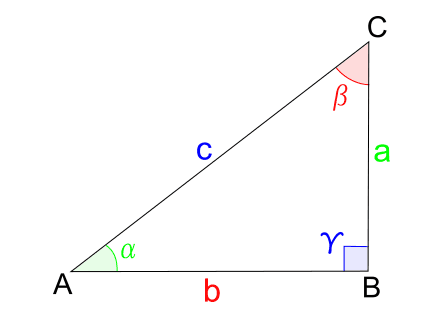
\includegraphics[width = 0.60\textwidth]{Immagini/Triangolo.PNG}
\end{center}
\subsection{Valori funzioni trigonometriche elementari}
\begin{tabular}{ |p{3cm}||p{3cm}|p{3cm}|p{3cm}|}
\hline
 \multicolumn{4}{|c|}{Valori funzioni trigonometriche} \\
 Valore(Rad) & Seno & Coseno & Tangente \\
 \hline
 0 & 0 & 1 & 0 \\
 \hline
 $\pi/12$ & $\frac{\sqrt{6}-\sqrt{2}}{4}$ &  $\frac{\sqrt{6}+\sqrt{2}}{4}$ & $2 - \sqrt{3}$ \\
 \hline
 $\pi/10$ & $\frac{\sqrt{5}-1}{4}$ & $\frac{\sqrt{10+ 2\sqrt{5}}}{4}$ &$\frac{\sqrt{25-10\sqrt{5}}}{4}$ \\
 \hline
 $\pi/8$ & $\frac{\sqrt{2- \sqrt{2}}}{2}$ & \textbf{$\frac{\sqrt{2+ \sqrt{2}}}{2}$} & $\sqrt{2}-1$ \\
 \hline
 $\pi/6$ & $1/2$ & $\frac{\sqrt{3}}{2}$ & $\frac{\sqrt{3}}{3}$ \\
 \hline
 $\pi/4$ & $\frac{\sqrt{2}}{2}$ & $\frac{\sqrt{2}}{2}$ & 1 \\
 \hline
 $\pi/3$ & $\frac{\sqrt{3}}{2}$ & $1/2$ & $\sqrt{3}$ \\
 \hline
 $\pi/2$ & $1$ & $0$ & $\pm \infty$ \\
 \hline
 $2/3 \pi$ & $\frac{\sqrt{3}}{2}$ & $-1/2$ & $-\sqrt{3}$ \\
 \hline
 $3/4 \pi$ & $\frac{\sqrt{2}}{2}$ & $-\frac{\sqrt{2}}{2}$ & -1 \\
 \hline
 $5/6 \pi$ & $1/2$ & $-\frac{\sqrt{3}}{2}$ & $-\frac{\sqrt{3}}{3}$ \\
 \hline
 $\pi$ & $0$ & $-1$ & $0$ \\
 \hline
 $7/6\pi$ & $-1/2$ & $-\frac{\sqrt{3}}{2}$ & $\frac{\sqrt{3}}{3}$ \\
 \hline
 $5/4\pi$ & $-\frac{\sqrt{2}}{2}$ & $-\frac{\sqrt{2}}{2}$ & 1 \\
 \hline
 $4/3\pi$ & $-\frac{\sqrt{3}}{2}$ & $-1/2$ & $\sqrt{3}$ \\
 \hline
 $3/2\pi$ & $-1$ & 0 & $\pm \infty$ \\
 \hline
 $5/3 \pi$ & $-\frac{\sqrt{3}}{2}$ & $1/2$ & $-\sqrt{3}$ \\
 \hline
 $7/4 \pi$ & $-\frac{\sqrt{2}}{2}$ & $\frac{\sqrt{2}}{2}$ & $-1$ \\
 \hline
 $11/6 \pi$ & $-1/2$ & $\frac{\sqrt{3}}{2}$ & $-\frac{\sqrt{3}}{3}$ \\
 \hline
 $2\pi$ & $0$ & $1$ & $0$ \\
 \hline
\end{tabular}
\newpage
\subsection{Soluzione generale per stabilire la validità di un omomorfismo}
\begin{figure}[h]
    \hspace*{-3cm}%
    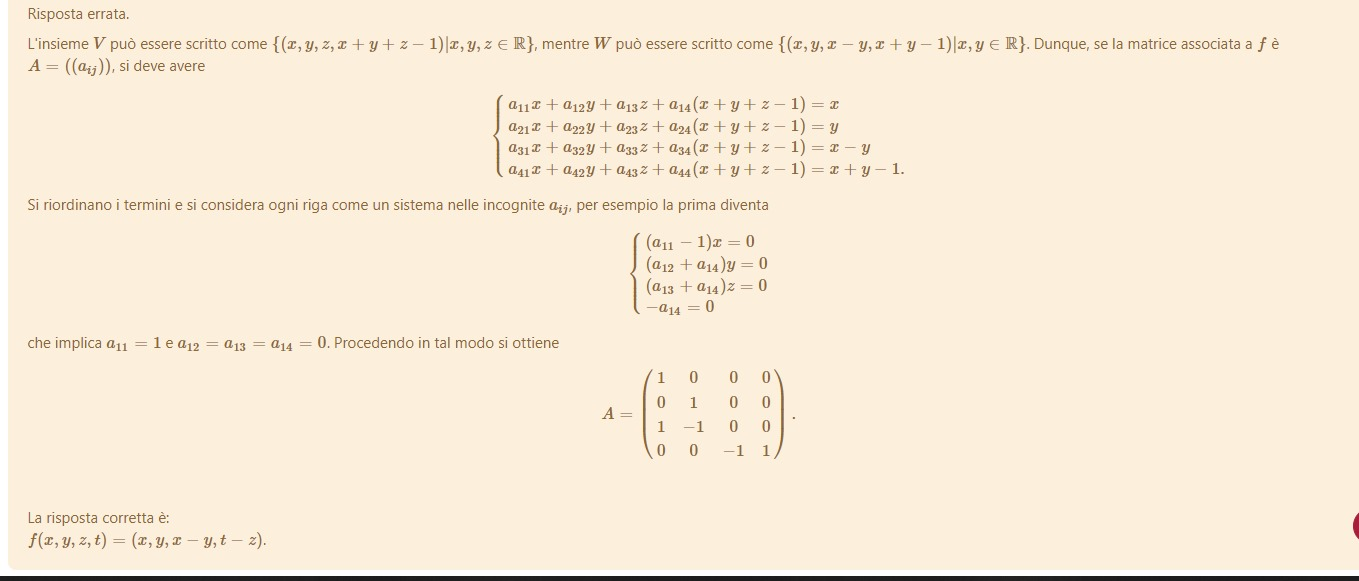
\includegraphics[width = 1.45\linewidth]{Immagini/Soluzione.jpeg}
    \hspace*{-3cm}%
    \vspace*{-1,4cm}%
\end{figure}
\subsection{Formule trigonometriche}
\subsubsection{Formule degli archi associati per seno e coseno}
\begin{itemize}
    \item $sin(\pi/2-\alpha) = cos(\alpha) \; \; \; cos(\pi/2 - \alpha) = sin(\alpha)$
    \item $sin(\pi/2 + \alpha) = cos(\alpha) \; \; \; cos(\pi/2 + \alpha) = -sin(\alpha)$
    \item $sin(\pi - \alpha) = sin(\alpha) \; \; \; cos(\pi - \alpha) = -cos(\alpha)$
    \item $sin(\pi + \alpha) = -sin(\alpha) \; \; \; cos (\pi + \alpha) = -cos(\alpha)$
    \item $sin(3/2\pi + \alpha) = -cos(\alpha) \; \; \; cos(3/2\pi + \alpha) = sin(\alpha)$
    \item $sin(3/2 \pi - \alpha) = -cos(\alpha) \; \; \; cos(3/2 \pi - \alpha) = -sin(\alpha)$
    \item $sin(-\alpha) = -sin(\alpha) \; \; \; cos(-\alpha) = cos(\alpha)$
\end{itemize}
\subsubsection{Formule di addizione e sottrazione}
\begin{itemize}
    \item $sin(\alpha + \beta) = sin(\alpha)cos(\beta)+cos(\alpha)sin(\beta)$
    \item $sin(\alpha - \beta) = sin(\alpha)cos(\beta)-cos(\alpha)sin(\beta)$
    \item $cos(\alpha+\beta) = cos(\alpha)cos(\beta)-sin(\alpha)sin(\beta)$
    \item $cos(\alpha-\beta) = cos(\alpha)cos(\beta)+sin(\alpha)sin(\beta)$
    \item $tan(\alpha+\beta) = \frac{tan(\alpha)+tan(\beta)}{1-tan(\alpha)tan(\beta)}$
    \item $tan(\alpha-\beta) = \frac{tan(\alpha)-tan(\beta)}{1+tan(\alpha)tan(\beta)}$
\end{itemize}

\end{para}
\end{document}